%&<tex>
\documentclass[notheorems,xcolor=dvipsnames]{beamer}
\usetheme{Rochester}
%\usefonttheme{serif}

%\usepackage[hmargin=2.5cm, vmargin=2cm]{geometry}
\usepackage{amssymb, mathtools, yhmath, graphicx}
\usepackage{standalone}
\usepackage[most]{tcolorbox}
%\usepackage{fontspec, type1cm, titlesec, titling, fancyhdr, tabularx}
%\usepackage{unicode-math}
\usepackage{float}
\usepackage{transparent}
\usepackage[normalem]{ulem}
\usepackage{bm}
\usepackage{array}
\usepackage{csquotes}
\usetikzlibrary{arrows}
\usepackage{soul}
\usepackage[normalem]{ulem}

%\usepackage{eulervm}

\usepackage{xpatch}
\usepackage{relsize}
\usepackage{scalerel}
\usepackage{stackengine}
\usepackage{gauss}
%\usepackage[abbreviations, per-mode=symbol]{siunitx}
\usepackage[CheckSingle, CJKmath]{xeCJK}
\usepackage{fontspec}
\defaultfontfeatures{Mapping=tex-text}
\usefonttheme{professionalfonts}
\usepackage{concmath}
%\usepackage{CJKulem}
%\usepackage{enumitem}
\usepackage{tikz}
\usetikzlibrary{calc, fit, backgrounds, arrows, arrows.meta, positioning, calc}
\usetikzlibrary{tikzmark}
\tikzset {
  overlay node/.style={
    anchor=base, outer sep=0mm, inner sep=0mm,
  }
}
\usepackage{minted}
\usepackage{python}
\usepackage{algorithm2e}
\usepackage{soul}
\usepackage{forest}
\usepackage{cancel}
\usepackage{svg}


\definecolor{mgray}{rgb}{0.85, 0.85, 0.85}
\colorlet{mgreen}{green!70!black}
\newmintinline{cpp}{bgcolor=mgray}
\def\codesize{\fontsize{9}{12}\selectfont}
\setmonofont[Mapping=]{Source Code Pro}
%\setmonofont[Contextuals={Alternate}]{Fira Code}
\setminted{fontsize=\codesize, linenos, frame=lines, mathescape, autogobble}
%\usemintedstyle{monokai}
%\usepackage{circuitikz}
%\setCJKmainfont[BoldFont=cwTex Q Hei]{cwTex Q Ming}
%\setCJKsansfont[BoldFont=cwTex Q Hei]{cwTex Q Ming}
%\setCJKmonofont[BoldFont=cwTex Q Hei]{cwTex Q Ming}
\setCJKmainfont[AutoFakeSlant,BoldFont=Noto Sans CJK TC Bold]{Noto Sans CJK TC}
\setCJKmonofont[AutoFakeSlant]{Noto Sans Mono CJK TC}
\newfontfamily\SHSTW{Noto Sans CJK TC}
% using the font "Source Han Sans TC VF" fucks up everything (since 2024). WHY?

\def\ofootnotesize{\fontsize{8}{12}}
\def\footnotesize{\fontsize{6}{8}\selectfont}
%\def\normalsize{\fontsize{12}{18}\selectfont}
%\def\large{\fontsize{14}{21}\selectfont}
%\def\Large{\fontsize{16}{24}\selectfont}
%\def\LARGE{\fontsize{18}{27}\selectfont}
%\def\huge{\fontsize{20}{30}\selectfont}

%\titleformat{\section}{\bf\Large}{\arabic{section}}{24pt}{}
%\titleformat{\subsection}{\large}{\arabic{subsection}.}{12pt}{}
%\titlespacing*{\subsection}{0pt}{0pt}{1.5ex}

%\usepackage{parskip}
%\parindent=24pt
%\parskip=1em

\setlength{\parskip}{\baselineskip} 
\usepackage{trimclip}
\DeclareRobustCommand\Longrightarrow{\NewRelbar\joinrel\Rightarrow}
\DeclareRobustCommand\Longleftarrow{\Leftarrow\joinrel\NewRelbar}

\makeatletter
\DeclareRobustCommand\NewRelbar{%
  \mathrel{%
    \mathpalette\@NewRelbar{}%
  }%
}
\newcommand*\@NewRelbar[2]{%
  % #1: math style
  % #2: unused
  \sbox0{$#1=$}%
  \sbox2{$#1\Rightarrow\m@th$}%
  \sbox4{$#1\Leftarrow\m@th$}%
  \clipbox{0pt 0pt \dimexpr(\wd2-.6\wd0) 0pt}{\copy2}%
  \kern-.2\wd0 %
  \clipbox{\dimexpr(\wd4-.6\wd0) 0pt 0pt 0pt}{\copy4}%
}
\makeatother



\newcommand{\img}{\mathsf{i}}
\newcommand{\ex}{\mathsf{e}}
\newcommand{\dD}{\mathrm{d}}
\newcommand{\dI}{\,\mathrm{d}}
\newcommand{\linearprog}[3][maximize]{%
\begin{array}{rl}
  \text{#1} & \kern 1em {#2} \\[8pt]
  \text{subject to} & {\renewcommand\arraystretch{1.1} #3}
\end{array}%
}

\newcommand\abs[1]{\left\lvert #1 \right\rvert}
\newcommand{\ord}{\mathcal{O}}
\newcommand{\fourier}{\mathcal{F}}
\newcommand*{\defeq}{\triangleq}
\renewcommand*{\sharp}{\mathlarger{\#}}
\newcommand*{\bZ}{\mathbb{Z}}
\newcommand*{\bF}{\mathbb{F}}
\newcommand*{\correspond}{\mathrel{\stackon[1.5pt]{=}{\stretchto{%
    \scalerel*[\widthof{=}]{\wedge}{\rule{1ex}{3ex}}}{0.5ex}}}}
\newcommand*{\Expect}{{\rm I\kern-.3em E}}
\newcommand{\ebtitle}{{\secname}}
\newcommand{\btitle}[1]{{\secname} -- #1}
\newcommand{\ectitle}{\subsecname}
\newcommand{\ctitle}[1]{{\subsecname} -- #1}
\newcommand{\disskip}[1][1]{\vspace*{-#1\parskip}}%
\renewcommand*{\sharp}{\mathlarger{\#}}
\newcommand{\tikzoverlay}[2]{\tikz[baseline, remember picture]{ \node[overlay node] (#1) {#2}}}%
\newcommand{\inc}[1]{\mintinline{cpp}{#1}}  % inline code
\renewcommand<>{\sout}[1]{
  \only#2{\beameroriginal{\sout}{#1}}
  \invisible#2{#1}
}

\theoremstyle{definition}
\newtheorem{theorem}{定理}
\newtheorem{lemma}{引理}
\newtheorem{property}{性質}
\newtheorem{corollary}{推論}
\newtheorem{conjecture}{猜想}
\newtheorem{problem}{題目}

%\colorlet{origintitlefg}{block title.fg}
%\setbeamercolor{origintitle}{use=block,fg=block title.fg,bg=block title.bg}
%\setbeamercolor{originbody}{use=block body,fg=block body.fg,bg=block body.bg}

\newtheorem{definition}{定義}
\BeforeBeginEnvironment{definition}{%
  \setbeamercolor{block title}{fg=white,bg=red!70!black}
  \setbeamercolor{block body}{fg=black, bg=block title.bg!10!bg}
}
\AfterEndEnvironment{definition}{
    \setbeamercolor{block title}{use=structure,fg=white,bg=structure.fg!75!black}
    \setbeamercolor{block body}{parent=normal text,use=block title,bg=block title.bg!10!bg}
}

\newenvironment{missue}{%
\setbeamercolor{block title}{bg=ForestGreen,fg=white}
\setbeamercolor{block body}{bg=blue!20!green!20,fg=black}
\begin{block}{\centering 問題}}{\end{block}}

\newenvironment{exercise}{%
\setbeamercolor{block title}{bg=ForestGreen,fg=white}
\setbeamercolor{block body}{bg=blue!20!green!20,fg=black}
\begin{block}{習題}}{\end{block}}

\renewenvironment{proof}{%
\begin{tcolorbox}[frame empty] {\bf 證明:}\ }{\end{tcolorbox}}

%\setbeamercovered{transparent}
%\usefonttheme[onlymath]{serif}
%\settowidth{\leftmargini}{\usebeamertemplate{itemize item}}

%\makeatletter
%\patchcmd\beamer@@tmpl@frametitle{\insertframetitle}{\insertsection-\insertframetitle}{}{}
%\makeatother

\setbeamertemplate{enumerate item}{%
  \usebeamercolor[bg]{item projected}%
  \raisebox{0.28ex}{\colorbox{bg}{\color{fg}\scriptsize\insertenumlabel}}%
}

\setbeamertemplate{itemize item}{%
  \usebeamercolor[bg]{item projected}%
  \raisebox{0.25ex}{\scriptsize$\blacksquare$}%
}

\AtBeginSection[]{
  \begin{frame}
    \tableofcontents[currentsection]
  \end{frame}
  \begin{frame}
  \vfill
  \centering
  \begin{beamercolorbox}[sep=6pt,center,shadow=true,rounded=true]{title}
    \usebeamerfont{title}\LARGE\insertsectionhead\par%
  \end{beamercolorbox}
  \vfill
  \end{frame}

}

\AtBeginSubsection[] {
  \begin{frame}{\secname}
    \vfill
    \centering
    \begin{beamercolorbox}[sep=6pt,center,shadow=true,rounded=true]{title}
      \usebeamerfont{title}\LARGE\insertsubsectionhead\par%
    \end{beamercolorbox}
    \vfill
  \end{frame}
}

\makeatletter
\let\save@measuring@true\measuring@true
\def\measuring@true{%
  \save@measuring@true
  \def\beamer@sortzero##1{\beamer@ifnextcharospec{\beamer@sortzeroread{##1}}{}}%
  \def\beamer@sortzeroread##1<##2>{}%
  \def\beamer@finalnospec{}%
}
\makeatother

\title{進階資料結構}
\author{邱翊均}

\newcommand{\brilliance}[1]{\raisebox{-.25\height}{\includesvg{images/brilliance_v2/svg/#1.svg}}}
\renewcommand*{\emph}[1]{{\bfseries #1}}
\setcounter{tocdepth}{1}

\begin{document}

% % \documentclass[standalone]{beamer}

% \begin{document}
\section{Section 1}

\begin{frame}{\btitle{Algorithm A}}
  \begin{enumerate}
    \item 123
    \item 456
    \item 789
  \end{enumerate}
\end{frame}

\begin{frame}{\btitle{Algorithm A}}
  
\begin{property}
  123123123123
\end{property}

\begin{theorem}
  Algorithm A is correct.
\end{theorem}

\end{frame}

\begin{frame}{\btitle{Algorithm A}}
  \begin{proof}
    \begin{enumerate}
      \item 123
      \item 456
      \item 789
    \end{enumerate}
  \end{proof}
\end{frame}

\begin{frame}{\btitle{Algorithm A}}

  \begin{problem}[King Game]
    King game king game.
  \end{problem}

\end{frame}

\begin{frame}{\btitle{Algorithm B}}
  \[ S_i = A_1 \oplus A_2 \oplus \ldots \oplus A_i \]
  \begin{figure}[H]
  \begin{tikzpicture}[scale=2]
  \tikzset{vertex/.style = {shape=circle,draw,minimum size=1.5em}}
  \tikzset{edge/.style = {-,> = latex'}}
  \node[vertex,fill=gray!40] (a) at (0, 0) {$0$};
  \only<4-> {
  \node[vertex,fill=gray!40] (b) at (1, 0) {$1$};
  }
  \only<1-3> {
  \node[vertex] (b) at (1, 0) {$1$};
  }
  \only<2-> {
  \node[vertex,fill=gray!40] (c) at (2, 0) {$2$};
  }
  \only<1> {
  \node[vertex] (c) at (2, 0) {$2$};
  }
  \only<6-> {
  \node[vertex,fill=gray!40] (d) at (3, 0) {$3$};
  }
  \only<1-5> {
  \node[vertex] (d) at (3, 0) {$3$};
  }
  \only<5-> {
  \node[vertex,fill=gray!40] (e) at (4, 0) {$4$};
  }
  \only<1-4> {
  \node[vertex] (e) at (4, 0) {$4$};
  }
  \only<3-> {
  \node[vertex,fill=gray!40] (f) at (5, 0) {$5$};
  }
  \only<1-2> {
  \node[vertex] (f) at (5, 0) {$5$};
  }
  \only<2-> {
    \draw[edge, bend right] (a) to (c);
  }
  \only<3-> {
    \draw[edge, bend right] (a) to (f);
  }
  \only<4-> {
    \draw[edge, bend left] (b) to (c);
  }
  \only<5-> {
    \draw[edge, bend left] (c) to (e);
  }
  \only<6-> {
    \draw[edge, bend right] (b) to (d);
  }
  \end{tikzpicture}
  \end{figure}
  \only<2> {詢問 $L = 1$, $R = 2$}
  \only<3> {詢問 $L = 1$, $R = 5$}
  \only<4> {詢問 $L = 2$, $R = 2$}
  \only<5> {詢問 $L = 3$, $R = 4$}
  \only<6> {詢問 $L = 2$, $R = 3$}
\end{frame}

\begin{frame}[fragile]{\btitle{Code}}
  \begin{minted}[linenos=false]{cpp}
    int main() {
      int a, b;
      std::cin >> a >> b;
      std::cout << a + b << "\n";
      return 0;
    }
  \end{minted}
\end{frame}

% \end{document}

\begin{frame}
    \titlepage
\end{frame}

\begin{frame}{講師簡介}
    \begin{itemize}
        \item 邱翊均 PixelCat
        \item 2022 全國賽場外觀眾
        \item IOI 2023、APIO 2023 銀牌
        \item ICPC PCkomachi 隊員
        \only<2-> {
            \item 因為想學習資料結構所以當資料結構講師
        }
    \end{itemize}
\end{frame}

\begin{frame}{大綱}
    \tableofcontents
\end{frame}

% abandoned

\section{很多很多線段樹}

\begin{frame}{\ebtitle}
    \begin{figure}[h!]
        \begin{center}
            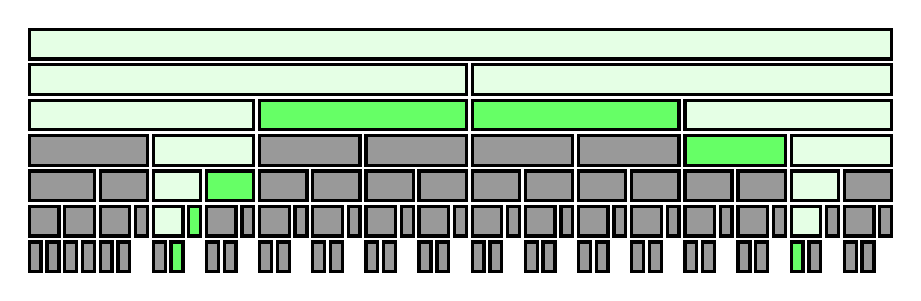
\begin{tikzpicture}[nodes = {transform shape}, scale=0.75]
                \pgfdeclarelayer{bg}
                \pgfsetlayers{bg, main}
                \tikzset{x={(0.1cm, 0cm)}, y={(0cm, 0.1cm)}}
            
                \draw [very thick, black, fill=white!90!green] (0, 0) rectangle (146, 5) node[black, midway, align=center] (nd0) {};
                \draw [very thick, black, fill=white!90!green] (0, -6) rectangle (74, -1) node[black, midway, align=center] (nd1) {};
                \draw [very thick, black, fill=white!90!green] (0, -12) rectangle (38, -7) node[black, midway, align=center] (nd3) {};
                \draw [very thick, black, fill=gray!80] (0, -18) rectangle (20, -13) node[black, midway, align=center] (nd7) {};
                \draw [very thick, black, fill=gray!80] (0, -24) rectangle (11, -19) node[black, midway, align=center] (nd15) {};
                \draw [very thick, black, fill=gray!80] (0, -30) rectangle (5, -25) node[black, midway, align=center] (nd31) {};
                \draw [very thick, black, fill=gray!80] (0, -36) rectangle (2, -31) node[black, midway, align=center] (nd63) {};
                \draw [very thick, black, fill=gray!80] (3, -36) rectangle (5, -31) node[black, midway, align=center] (nd64) {};
                \draw [very thick, black, fill=gray!80] (6, -30) rectangle (11, -25) node[black, midway, align=center] (nd32) {};
                \draw [very thick, black, fill=gray!80] (6, -36) rectangle (8, -31) node[black, midway, align=center] (nd65) {};
                \draw [very thick, black, fill=gray!80] (9, -36) rectangle (11, -31) node[black, midway, align=center] (nd66) {};
                \draw [very thick, black, fill=gray!80] (12, -24) rectangle (20, -19) node[black, midway, align=center] (nd16) {};
                \draw [very thick, black, fill=gray!80] (12, -30) rectangle (17, -25) node[black, midway, align=center] (nd33) {};
                \draw [very thick, black, fill=gray!80] (12, -36) rectangle (14, -31) node[black, midway, align=center] (nd67) {};
                \draw [very thick, black, fill=gray!80] (15, -36) rectangle (17, -31) node[black, midway, align=center] (nd68) {};
                \draw [very thick, black, fill=gray!80] (18, -30) rectangle (20, -25) node[black, midway, align=center] (nd34) {};
                \draw [very thick, black, fill=white!90!green] (21, -18) rectangle (38, -13) node[black, midway, align=center] (nd8) {};
                \draw [very thick, black, fill=white!90!green] (21, -24) rectangle (29, -19) node[black, midway, align=center] (nd17) {};
                \draw [very thick, black, fill=white!90!green] (21, -30) rectangle (26, -25) node[black, midway, align=center] (nd35) {};
                \draw [very thick, black, fill=gray!80] (21, -36) rectangle (23, -31) node[black, midway, align=center] (nd71) {};
                \draw [very thick, black, fill=white!40!green] (24, -36) rectangle (26, -31) node[black, midway, align=center] (nd72) {};
                \draw [very thick, black, fill=white!40!green] (27, -30) rectangle (29, -25) node[black, midway, align=center] (nd36) {};
                \draw [very thick, black, fill=white!40!green] (30, -24) rectangle (38, -19) node[black, midway, align=center] (nd18) {};
                \draw [very thick, black, fill=gray!80] (30, -30) rectangle (35, -25) node[black, midway, align=center] (nd37) {};
                \draw [very thick, black, fill=gray!80] (30, -36) rectangle (32, -31) node[black, midway, align=center] (nd75) {};
                \draw [very thick, black, fill=gray!80] (33, -36) rectangle (35, -31) node[black, midway, align=center] (nd76) {};
                \draw [very thick, black, fill=gray!80] (36, -30) rectangle (38, -25) node[black, midway, align=center] (nd38) {};
                \draw [very thick, black, fill=white!40!green] (39, -12) rectangle (74, -7) node[black, midway, align=center] (nd4) {};
                \draw [very thick, black, fill=gray!80] (39, -18) rectangle (56, -13) node[black, midway, align=center] (nd9) {};
                \draw [very thick, black, fill=gray!80] (39, -24) rectangle (47, -19) node[black, midway, align=center] (nd19) {};
                \draw [very thick, black, fill=gray!80] (39, -30) rectangle (44, -25) node[black, midway, align=center] (nd39) {};
                \draw [very thick, black, fill=gray!80] (39, -36) rectangle (41, -31) node[black, midway, align=center] (nd79) {};
                \draw [very thick, black, fill=gray!80] (42, -36) rectangle (44, -31) node[black, midway, align=center] (nd80) {};
                \draw [very thick, black, fill=gray!80] (45, -30) rectangle (47, -25) node[black, midway, align=center] (nd40) {};
                \draw [very thick, black, fill=gray!80] (48, -24) rectangle (56, -19) node[black, midway, align=center] (nd20) {};
                \draw [very thick, black, fill=gray!80] (48, -30) rectangle (53, -25) node[black, midway, align=center] (nd41) {};
                \draw [very thick, black, fill=gray!80] (48, -36) rectangle (50, -31) node[black, midway, align=center] (nd83) {};
                \draw [very thick, black, fill=gray!80] (51, -36) rectangle (53, -31) node[black, midway, align=center] (nd84) {};
                \draw [very thick, black, fill=gray!80] (54, -30) rectangle (56, -25) node[black, midway, align=center] (nd42) {};
                \draw [very thick, black, fill=gray!80] (57, -18) rectangle (74, -13) node[black, midway, align=center] (nd10) {};
                \draw [very thick, black, fill=gray!80] (57, -24) rectangle (65, -19) node[black, midway, align=center] (nd21) {};
                \draw [very thick, black, fill=gray!80] (57, -30) rectangle (62, -25) node[black, midway, align=center] (nd43) {};
                \draw [very thick, black, fill=gray!80] (57, -36) rectangle (59, -31) node[black, midway, align=center] (nd87) {};
                \draw [very thick, black, fill=gray!80] (60, -36) rectangle (62, -31) node[black, midway, align=center] (nd88) {};
                \draw [very thick, black, fill=gray!80] (63, -30) rectangle (65, -25) node[black, midway, align=center] (nd44) {};
                \draw [very thick, black, fill=gray!80] (66, -24) rectangle (74, -19) node[black, midway, align=center] (nd22) {};
                \draw [very thick, black, fill=gray!80] (66, -30) rectangle (71, -25) node[black, midway, align=center] (nd45) {};
                \draw [very thick, black, fill=gray!80] (66, -36) rectangle (68, -31) node[black, midway, align=center] (nd91) {};
                \draw [very thick, black, fill=gray!80] (69, -36) rectangle (71, -31) node[black, midway, align=center] (nd92) {};
                \draw [very thick, black, fill=gray!80] (72, -30) rectangle (74, -25) node[black, midway, align=center] (nd46) {};
                \draw [very thick, black, fill=white!90!green] (75, -6) rectangle (146, -1) node[black, midway, align=center] (nd2) {};
                \draw [very thick, black, fill=white!40!green] (75, -12) rectangle (110, -7) node[black, midway, align=center] (nd5) {};
                \draw [very thick, black, fill=gray!80] (75, -18) rectangle (92, -13) node[black, midway, align=center] (nd11) {};
                \draw [very thick, black, fill=gray!80] (75, -24) rectangle (83, -19) node[black, midway, align=center] (nd23) {};
                \draw [very thick, black, fill=gray!80] (75, -30) rectangle (80, -25) node[black, midway, align=center] (nd47) {};
                \draw [very thick, black, fill=gray!80] (75, -36) rectangle (77, -31) node[black, midway, align=center] (nd95) {};
                \draw [very thick, black, fill=gray!80] (78, -36) rectangle (80, -31) node[black, midway, align=center] (nd96) {};
                \draw [very thick, black, fill=gray!80] (81, -30) rectangle (83, -25) node[black, midway, align=center] (nd48) {};
                \draw [very thick, black, fill=gray!80] (84, -24) rectangle (92, -19) node[black, midway, align=center] (nd24) {};
                \draw [very thick, black, fill=gray!80] (84, -30) rectangle (89, -25) node[black, midway, align=center] (nd49) {};
                \draw [very thick, black, fill=gray!80] (84, -36) rectangle (86, -31) node[black, midway, align=center] (nd99) {};
                \draw [very thick, black, fill=gray!80] (87, -36) rectangle (89, -31) node[black, midway, align=center] (nd100) {};
                \draw [very thick, black, fill=gray!80] (90, -30) rectangle (92, -25) node[black, midway, align=center] (nd50) {};
                \draw [very thick, black, fill=gray!80] (93, -18) rectangle (110, -13) node[black, midway, align=center] (nd12) {};
                \draw [very thick, black, fill=gray!80] (93, -24) rectangle (101, -19) node[black, midway, align=center] (nd25) {};
                \draw [very thick, black, fill=gray!80] (93, -30) rectangle (98, -25) node[black, midway, align=center] (nd51) {};
                \draw [very thick, black, fill=gray!80] (93, -36) rectangle (95, -31) node[black, midway, align=center] (nd103) {};
                \draw [very thick, black, fill=gray!80] (96, -36) rectangle (98, -31) node[black, midway, align=center] (nd104) {};
                \draw [very thick, black, fill=gray!80] (99, -30) rectangle (101, -25) node[black, midway, align=center] (nd52) {};
                \draw [very thick, black, fill=gray!80] (102, -24) rectangle (110, -19) node[black, midway, align=center] (nd26) {};
                \draw [very thick, black, fill=gray!80] (102, -30) rectangle (107, -25) node[black, midway, align=center] (nd53) {};
                \draw [very thick, black, fill=gray!80] (102, -36) rectangle (104, -31) node[black, midway, align=center] (nd107) {};
                \draw [very thick, black, fill=gray!80] (105, -36) rectangle (107, -31) node[black, midway, align=center] (nd108) {};
                \draw [very thick, black, fill=gray!80] (108, -30) rectangle (110, -25) node[black, midway, align=center] (nd54) {};
                \draw [very thick, black, fill=white!90!green] (111, -12) rectangle (146, -7) node[black, midway, align=center] (nd6) {};
                \draw [very thick, black, fill=white!40!green] (111, -18) rectangle (128, -13) node[black, midway, align=center] (nd13) {};
                \draw [very thick, black, fill=gray!80] (111, -24) rectangle (119, -19) node[black, midway, align=center] (nd27) {};
                \draw [very thick, black, fill=gray!80] (111, -30) rectangle (116, -25) node[black, midway, align=center] (nd55) {};
                \draw [very thick, black, fill=gray!80] (111, -36) rectangle (113, -31) node[black, midway, align=center] (nd111) {};
                \draw [very thick, black, fill=gray!80] (114, -36) rectangle (116, -31) node[black, midway, align=center] (nd112) {};
                \draw [very thick, black, fill=gray!80] (117, -30) rectangle (119, -25) node[black, midway, align=center] (nd56) {};
                \draw [very thick, black, fill=gray!80] (120, -24) rectangle (128, -19) node[black, midway, align=center] (nd28) {};
                \draw [very thick, black, fill=gray!80] (120, -30) rectangle (125, -25) node[black, midway, align=center] (nd57) {};
                \draw [very thick, black, fill=gray!80] (120, -36) rectangle (122, -31) node[black, midway, align=center] (nd115) {};
                \draw [very thick, black, fill=gray!80] (123, -36) rectangle (125, -31) node[black, midway, align=center] (nd116) {};
                \draw [very thick, black, fill=gray!80] (126, -30) rectangle (128, -25) node[black, midway, align=center] (nd58) {};
                \draw [very thick, black, fill=white!90!green] (129, -18) rectangle (146, -13) node[black, midway, align=center] (nd14) {};
                \draw [very thick, black, fill=white!90!green] (129, -24) rectangle (137, -19) node[black, midway, align=center] (nd29) {};
                \draw [very thick, black, fill=white!90!green] (129, -30) rectangle (134, -25) node[black, midway, align=center] (nd59) {};
                \draw [very thick, black, fill=white!40!green] (129, -36) rectangle (131, -31) node[black, midway, align=center] (nd119) {};
                \draw [very thick, black, fill=gray!80] (132, -36) rectangle (134, -31) node[black, midway, align=center] (nd120) {};
                \draw [very thick, black, fill=gray!80] (135, -30) rectangle (137, -25) node[black, midway, align=center] (nd60) {};
                \draw [very thick, black, fill=gray!80] (138, -24) rectangle (146, -19) node[black, midway, align=center] (nd30) {};
                \draw [very thick, black, fill=gray!80] (138, -30) rectangle (143, -25) node[black, midway, align=center] (nd61) {};
                \draw [very thick, black, fill=gray!80] (138, -36) rectangle (140, -31) node[black, midway, align=center] (nd123) {};
                \draw [very thick, black, fill=gray!80] (141, -36) rectangle (143, -31) node[black, midway, align=center] (nd124) {};
                \draw [very thick, black, fill=gray!80] (144, -30) rectangle (146, -25) node[black, midway, align=center] (nd62) {};
            \end{tikzpicture}
        \end{center}
        \caption{$N = 49$,區間查詢 $[9, 44]$(Source:2024 基礎資結投影片)}
    \end{figure}
\end{frame}

\begin{frame}{\btitle{前言}}
    你一定寫過線段樹!

    線段樹普及,大家都會用線段樹砸區間操作 \\
    你都用線段樹做過什麼事情?
\end{frame}

\begin{frame}{\btitle{前言}}
    \begin{itemize}
        \item \tikzoverlay{nd0}{}區間求和、極值、最大公因數
        \item \tikzoverlay{nd1}{}單點修改、區間加值
        \item \tikzoverlay{nd2}{}歷史版本的區間和
        \item \tikzoverlay{nd3}{}區間最大連續和
        \item \tikzoverlay{nd4}{}區間 MEX、矩形覆蓋面積
        \item \tikzoverlay{nd5}{}靜態區間和 \brilliance{blunder}
    \end{itemize}

    \begin{tikzpicture}[remember picture, overlay]
        \node[right=6cm of nd0, anchor=base west] {(一般線段樹)};
        \node[right=6cm of nd1, anchor=base west] {(懶人標記)};
        \node[right=6cm of nd2, anchor=base west] {(持久化)};
        \node[right=6cm of nd3, anchor=base west] {(分治)};
        \node[right=6cm of nd4, anchor=base west] {(離線、掃描線)};
        \node[right=6cm of nd5, anchor=base west] {(拜託不要)};
    \end{tikzpicture}
\end{frame}

\begin{frame}{\btitle{前言}}
    不只是區間詢問,線段樹可以有更多花樣!

    \begin{itemize}
        \item 李超線段樹
        \item 時間線段樹
        \item 線段樹優化建圖
    \end{itemize}
\end{frame}


\subsection{李超線段樹}

\begin{frame}{\ectitle}
    \begin{problem}[動態凸包]
        現在有 $Q$ 個操作,每個操作會是以下兩種中的一種:

        \begin{itemize}
            \item 加入一條直線 $y = mx + k$
            \item 詢問在 $x = t$ 處最大的 $y$ 值
        \end{itemize}

        \begin{itemize}
            \item $1\le Q \le 10^5$
            \item $|m|, |k| \le 10^9$
            \item $1 \le t \le 10^5$
        \end{itemize}
    \end{problem}
\end{frame}

\begin{frame}{\ectitle}
    用 set 維護上凸包上的線段,維護線段控制的左右界,每次加入直線先搜他控制的區間,往左右殺掉其他線段,查詢的時候二分搜是哪條線段代值進去。注意 iterator 使用、全整求線交點......

    太麻煩了,而且常數不小\sout{,而且我沒寫過} \\
    有沒有簡單一點的辦法?
\end{frame}

\begin{frame}{\ectitle}
    李超線段樹:
    \begin{itemize}
        \item 對要查詢的\yum{值域}開線段樹,葉子代表單一一個 $x$ 的值
        \item 每個節點存\yum{一條}對\yum{中點}來說 $y$ 最大的直線
        \begin{itemize}
            \item 對中點一定是有用的
            \item 可能還對這個區間的其他一部分有用
        \end{itemize}
    \end{itemize}
\end{frame}

\begin{frame}{\ctitle{插入直線}}
    原本節點上有一條直線 \\
    這次詢問想插入另外一條直線

    一個節點只能存一條線
    誰要留下來?另一條線要去哪裡?
\end{frame}

\begin{frame}{\ctitle{插入直線}}
    \only<1> {
        \begin{centikz}
            \draw[color=gray, dashed] (-5, 0) -- (-5, 5);
            \draw[color=gray, dashed] ( 0, 0) -- ( 0, 5);
            \draw[color=gray, dashed] ( 5, 0) -- ( 5, 5);
            \node[color=gray, anchor=north] at (-5, -0.2) {$L$};
            \node[color=gray, anchor=north] at ( 0, -0.2) {$M = \frac{L + R}{2}$};
            \node[color=gray, anchor=north] at ( 5, -0.2) {$R$};
            \draw[color=black, very thick] plot[domain=-5:5] (\x,{0.3 * \x + 2.8});
            \draw[color=black, very thick] plot[domain=-5:5] (\x,{-0.2 * \x + 2.1});
        \end{centikz}
    }

    \only<2> {
        \begin{centikz}
            \draw[color=gray, dashed] (-5, 0) -- (-5, 5);
            \draw[color=gray, dashed] ( 0, 0) -- ( 0, 5);
            \draw[color=gray, dashed] ( 5, 0) -- ( 5, 5);
            \node[color=gray, anchor=north] at (-5, -0.2) {$L$};
            \node[color=gray, anchor=north] at ( 0, -0.2) {$M = \frac{L + R}{2}$};
            \node[color=gray, anchor=north] at ( 5, -0.2) {$R$};
            \draw[color=black, very thick] plot[domain=-5:5] (\x,{-0.2 * \x + 2.1});
            \draw[color=Lime, very thick] plot[domain=-5:5] (\x,{0.3 * \x + 2.8});
            \node[anchor=south west] at (0, 3) {\brilliance{best}};
        \end{centikz}
    }

    \only<3> {
        \begin{centikz}
            \draw[color=gray, dashed] (-5, 0) -- (-5, 5);
            \draw[color=gray, dashed] ( 0, 0) -- ( 0, 5);
            \draw[color=gray, dashed] ( 5, 0) -- ( 5, 5);
            \node[color=gray, anchor=north] at (-5, -0.2) {$L$};
            \node[color=gray, anchor=north] at ( 0, -0.2) {$M = \frac{L + R}{2}$};
            \node[color=gray, anchor=north] at ( 5, -0.2) {$R$};
            
            \draw[color=DarkSeaGreen, very thick] plot[domain=-5:-1.4] (\x,{-0.2 * \x + 2.1});
            \draw[color=Red, very thick] plot[domain=-1.4:5] (\x,{-0.2 * \x + 2.1});
            \node[anchor=south] at (-3.2, 2.84) {\brilliance{good}};
            \node[anchor=south] at (2.5, 1.7) {\brilliance{incorrect}};
            
            \draw[color=Lime, very thick] plot[domain=-5:5] (\x,{0.3 * \x + 2.8});
            \node[anchor=south west] at (0, 3) {\brilliance{best}};
        \end{centikz}
    }
\end{frame}

\begin{frame}{\ctitle{插入直線}}
    \only<1> {
        \begin{centikz}
            \draw[color=gray, dashed] (-5, 0) -- (-5, 5);
            \draw[color=gray, dashed] ( 0, 0) -- ( 0, 5);
            \draw[color=gray, dashed] ( 5, 0) -- ( 5, 5);
            \node[color=gray, anchor=north] at (-5, -0.2) {$L$};
            \node[color=gray, anchor=north] at ( 0, -0.2) {$M = \frac{L + R}{2}$};
            \node[color=gray, anchor=north] at ( 5, -0.2) {$R$};
            \draw[color=black, very thick] plot[domain=-5:5] (\x,{0.3 * \x + 2.1});
            \draw[color=black, very thick] plot[domain=-5:5] (\x,{-0.2 * \x + 2.8});
        \end{centikz}
    }

    \only<2> {
        \begin{centikz}
            \draw[color=gray, dashed] (-5, 0) -- (-5, 5);
            \draw[color=gray, dashed] ( 0, 0) -- ( 0, 5);
            \draw[color=gray, dashed] ( 5, 0) -- ( 5, 5);
            \node[color=gray, anchor=north] at (-5, -0.2) {$L$};
            \node[color=gray, anchor=north] at ( 0, -0.2) {$M = \frac{L + R}{2}$};
            \node[color=gray, anchor=north] at ( 5, -0.2) {$R$};
            \draw[color=black, very thick] plot[domain=-5:5] (\x,{0.3 * \x + 2.1});
            \draw[color=Lime, very thick] plot[domain=-5:5] (\x,{-0.2 * \x + 2.8});
            \node[anchor=south west] at (0, 2.8) {\brilliance{best}};
        \end{centikz}
    }

    \only<3> {
        \begin{centikz}
            \draw[color=gray, dashed] (-5, 0) -- (-5, 5);
            \draw[color=gray, dashed] ( 0, 0) -- ( 0, 5);
            \draw[color=gray, dashed] ( 5, 0) -- ( 5, 5);
            \node[color=gray, anchor=north] at (-5, -0.2) {$L$};
            \node[color=gray, anchor=north] at ( 0, -0.2) {$M = \frac{L + R}{2}$};
            \node[color=gray, anchor=north] at ( 5, -0.2) {$R$};

            \draw[color=Red, very thick] plot[domain=-5:1.4] (\x,{0.3 * \x + 2.1});
            \draw[color=DarkSeaGreen, very thick] plot[domain=1.4:5] (\x,{0.3 * \x + 2.1});
            \node[anchor=south] at (-2.5, 1.45) {\brilliance{incorrect}};
            \node[anchor=south] at (3.2, 3.16) {\brilliance{good}};

            \draw[color=Lime, very thick] plot[domain=-5:5] (\x,{-0.2 * \x + 2.8});
            \node[anchor=south west] at (0, 2.8) {\brilliance{best}};
        \end{centikz}
    }
\end{frame}

\begin{frame}{\ctitle{插入直線}}
    一條直線在中點輸掉之後不能直接扔掉,因為他還沒輸光,區間內某些 $x$ 的範圍可能還需要他

    在中點輸掉的話,一定也會在左右其中一邊輸光 \\
    只有其中一邊可能還會需要用到這條直線,遞迴把他交給線段樹上那半邊的子樹處置,另外半邊已經不需要他了

    到葉子還輸的話那這條線徹底不會被任何人需要
\end{frame}

\begin{frame}{\ctitle{插入直線}}
    \only<1> {
        \begin{centikz}
            \draw[color=gray, dashed] (-5, 0) -- (-5, 5);
            \draw[color=gray, dashed] ( 0, 0) -- ( 0, 5);
            \draw[color=gray, dashed] ( 5, 0) -- ( 5, 5);
            \node[color=gray, anchor=north] at (-5, -0.2) {$L$};
            \node[color=gray, anchor=north] at ( 0, -0.2) {$M = \frac{L + R}{2}$};
            \node[color=gray, anchor=north] at ( 5, -0.2) {$R$};
            \draw[color=black, very thick] plot[domain=-5:5] (\x,{0.3 * \x + 2.8});
            \draw[color=black, very thick] plot[domain=-5:5] (\x,{-0.2 * \x + 2.1});
        \end{centikz}
    }

    \only<2> {
        \begin{centikz}
            \draw[color=gray, dashed] (-5, 0) -- (-5, 5);
            \draw[color=gray, dashed] ( 0, 0) -- ( 0, 5);
            \draw[color=gray, dashed] ( 5, 0) -- ( 5, 5);
            \node[color=gray, anchor=north] at (-5, -0.2) {$L$};
            \node[color=gray, anchor=north] at ( 0, -0.2) {$M = \frac{L + R}{2}$};
            \node[color=gray, anchor=north] at ( 5, -0.2) {$R$};
            \draw[color=DarkSeaGreen, very thick] plot[domain=-5:0] (\x,{-0.2 * \x + 2.1});
            \draw[color=Lime, very thick] plot[domain=-5:5] (\x,{0.3 * \x + 2.8});
            \node[anchor=south west] at (0, 3) {\brilliance{best}};
            \node[anchor=south] at (-2.5, 2.7) {\brilliance{forced}};
        \end{centikz}
    }

    \only<3> {
        \begin{centikz}
            \draw[color=gray, dashed] (-5, 0) -- (-5, 5);
            \draw[color=gray, dashed] ( 0, 0) -- ( 0, 5);
            \draw[color=gray, dashed] ( 5, 0) -- ( 5, 5);
            \node[color=gray, anchor=north] at (-5, -0.2) {$L$};
            \node[color=gray, anchor=north] at ( 0, -0.2) {$M = \frac{L + R}{2}$};
            \node[color=gray, anchor=north] at ( 5, -0.2) {$R$};
            \draw[color=black, very thick] plot[domain=-5:5] (\x,{0.3 * \x + 2.1});
            \draw[color=black, very thick] plot[domain=-5:5] (\x,{-0.2 * \x + 2.8});
        \end{centikz}
    }

    \only<4> {
        \begin{centikz}
            \draw[color=gray, dashed] (-5, 0) -- (-5, 5);
            \draw[color=gray, dashed] ( 0, 0) -- ( 0, 5);
            \draw[color=gray, dashed] ( 5, 0) -- ( 5, 5);
            \node[color=gray, anchor=north] at (-5, -0.2) {$L$};
            \node[color=gray, anchor=north] at ( 0, -0.2) {$M = \frac{L + R}{2}$};
            \node[color=gray, anchor=north] at ( 5, -0.2) {$R$};
            \draw[color=DarkSeaGreen, very thick] plot[domain=0:5] (\x,{0.3 * \x + 2.1});
            \draw[color=Lime, very thick] plot[domain=-5:5] (\x,{-0.2 * \x + 2.8});
            \node[anchor=south west] at (0, 2.8) {\brilliance{best}};
            \node[anchor=south] at (2.5, 2.95) {\brilliance{forced}};
        \end{centikz}
    }
\end{frame}

\begin{frame}{\ctitle{插入直線}}
    從根節點出發,到葉節點為止:

    \begin{itemize}
        \item 代中點 $x$ 座標比較兩條直線,贏家留在節點上
        \item 比較兩條直線的斜率
        \begin{itemize}
            \item 如果贏家的斜率比較\strong{大},輸家往\strong{左}子樹遞迴插入
            \item 如果贏家的斜率比較\strong{小},輸家往\strong{右}子樹遞迴插入
        \end{itemize}
    \end{itemize}

    一直往子樹丟包直線\\
    時間複雜度 $O(\text{線段樹高}) = O(\log N)$
\end{frame}

\begin{frame}{\ctitle{單點查詢}}
    直線被扔到隔壁節點,代表這個範圍的 $x$ 全都用不到這條直線 \\
    一個 $x$ 可能用到的直線,都存在他的祖先們身上

    \begin{itemize}
        \item 找到代表這個 $x$ 值的葉子
        \item 檢查所有祖先存的直線,每個都代一次,回答最大的 $y$
    \end{itemize}

    時間複雜度 $O(\text{線段樹高}) = O(\log N)$
\end{frame}

\begin{frame}[fragile]{\ctitle{實做}}
    包裝直線作為函數使用
    
    \begin{minted}{cpp}
        struct Line {
            int a, b;  // y = ax + b
            Line(int _a = 0, int _b = 0): a(_a), b(_b) {}
            int operator()(int x) { return a * x + b; }
        };
    \end{minted}
\end{frame}

\begin{frame}[fragile]{\ctitle{實做}}
    插入直線

    \begin{itemize}
        \item 代中點 $x$ 座標比較兩條直線,贏家留在節點上
        \item 比較兩條直線的斜率
        \item 遞迴插入
    \end{itemize}
    
    \begin{minted}{cpp}
        void insert(int id, int l, int r, Line ln) {
            int m = (l + r) / 2;
            if(lns[id](m) < ln(m)) swap(lns[id], ln);
            if(l == r) return;
            if(lns[id].a > ln.a) insert(L(id), l, m, ln);
            else insert(R(id), m + 1, r, ln);
        }
    \end{minted}
\end{frame}

\begin{frame}[fragile]{\ctitle{實做}}
    單點查詢

    \begin{itemize}
        \item 找到代表這個 $x$ 值的葉子
        \item 檢查所有祖先存的直線,每個都代一次,回答最大的 $y$
    \end{itemize}
    
    \begin{minted}{cpp}
        int qry(int id, int l, int r, int x) {
            int m = (l + r) / 2;
            int res = lns[id](x);
            if(l == r) return res;
            if(x <= m) res = max(res, qry(L(id), l, m, x));
            else res = max(res, qry(R(id), m + 1, r, x));
            return res;
        }
    \end{minted}
\end{frame}

\begin{frame}{\ctitle{座標壓縮}}
    \begin{problem}[Line Add Get Min,Library Checker]
        你有 $N$ 條直線 $y = a_i x + b_i$。請你處理 $Q$ 個詢問:

        \begin{itemize}
            \item 加入一條直線 $y = ax + b$
            \item 詢問 $x = p$ 處最小的 $y$ 值
        \end{itemize}

        \begin{itemize}
            \item $1 \le N, Q \le 2 \times 10^5$
            \item $|a_i|, |p| \le 10^9$ \only<2>{\yum{???!!}}
            \item $|b_i| \le 10^{18}$
        \end{itemize}
    \end{problem}
\end{frame}

\begin{frame}{\ctitle{座標壓縮}}
    剛剛對 $x$ 的值域 $1, 2, \dots, 10^5$ 開線段樹

    現在事先收集會被詢問到的 $x$ 座標 \\
    對會被問到的 $x$ 開線段樹

    詢問是浮點數的時候也可以
\end{frame}

\begin{frame}{\ctitle{座標壓縮}}
    如果事先不知道詢問位置呢?

    \only<2> {
        動態開點,用不到的節點不要理他
    }
\end{frame}

\begin{frame}{\ctitle{插入線段}}
    如果插入的不是直線,而是有左右範圍限制的線段呢?

    \todo 插圖
\end{frame}

\begin{frame}{\ctitle{插入線段}}
    一般線段樹是怎麼做區間修改的?
    \only<2-> {
        \\找 $O(\log N)$ 個節點覆蓋詢問的區間,修改那些節點
    }

    \only<3-> {
        找 $O(\log N)$ 個節點覆蓋線段範圍,對那些節點插入直線
    }

    \only<4-> {
        時間複雜度:插入一次 $O(\log N)$,總共 $O(\log^2N)$
    }
\end{frame}

\begin{frame}{\ctitle{應用}}
    \begin{itemize}
        \item 斜率優化 \emoji{white_check_mark}
        \item<2> 四邊形優化 \emoji{white_check_mark}
    \end{itemize}

    \only<2> {
        不只是直線,有\strong{優超性}的函數都可以
    }
\end{frame}

% todo: li-chao segtree extensions

\newcommand{\InlineCode}[1]{\mintinline{cpp}|#1|}

\section{時間線段樹}

\iffalse

\begin{frame}{\ebtitle}
    如果要一句話解釋時間線段樹:\\
    「時間線段樹是一種用 stack 模擬 set 的辦法」

    \only<2> {
        (沒有解釋到半點 \emoji{pensive})
    }
\end{frame}

\fi

\begin{frame}{\ebtitle}
    \only<1,3> {
        時間線段樹想解決「操作有時效性」的問題
        
        你想要在未來的某個時間取消這次操作 \\
        但資料結構只有支援你做新的操作、和取消\yum{上一次}操作
    }

    \only<2> {
        例如:
        \begin{itemize}
            \item 你有一個 stack,想要加新元素、和移除任意久以前加進去的東西。但是 stack 只支援移除\yum{上一次}加進去的元素
            \item 你有一個併查集,想要加新的邊、和移除任意一條加過的邊。但是併查集只支援刪除\yum{上一次}加進去的邊
        \end{itemize}
    }

    \only<3> {
        如果\yum{操作沒有順序性}的話\\
        可以以複雜度乘 $O(\log Q)$ 的代價,使用時間線段樹支援 $Q$ 次這類操作
    }
\end{frame}

\begin{frame}{\ebtitle}
    線段樹的實做框架(講義第 79 頁)

    \begin{itemize}
        \item 先收集每個操作的有效時間段,加到時間線段樹裡
        \item 遍歷時間線段樹重現所有操作
    \end{itemize}
\end{frame}

\begin{frame}{\ebtitle}
    \begin{problem}[【Gate】這個笑容由我來守護 - EXTREME,TIOJ 1903]
        給定一張 $N$ 個點的無向圖,一開始圖上有 $M$ 條邊。

        現在有 $Q$ 個操作,每個操作會是以下兩種中的一種:
        
        \begin{itemize}
            \item 增加一條連接著編號 $A_i$ 與編號 $B_i$ 的邊。
            \item 刪除一條連接著編號 $A_i$ 與編號 $B_i$ 的邊(保證這條邊是存在的)。
        \end{itemize}

        每次操作完後請輸出當前的連通塊數量。

        \begin{itemize}
            \item $1\le N\le 5\times 10^5$。
            \item $Q\le 5\times 10^5$。
        \end{itemize}
    \end{problem}
\end{frame}

\begin{frame}{\ebtitle}
    \begin{itemize}
        \item 時間線段樹對「操作時間」開一棵線段樹
        \item 每個節點存一些操作
        \item 事先收集所有操作,在線段樹上的一些節點存起來
        \item \InlineCode{traversal} 遍歷線段樹,重現所有操作
    \end{itemize}
\end{frame}

\begin{frame}{\ebtitle}
    如果開始到結束經歷 $Q$ 次加邊或刪邊 \\
    對這 $Q$ 個時間點開線段樹 \\
    每個葉子的所有祖先存的所有邊,會是這個時間點應該要活著的所有邊
\end{frame}

\begin{frame}[fragile]{\ebtitle}
    加入操作:像區間修改一樣,把要加的邊紀錄在被修改到的節點上
    \begin{minted}[linenos=false]{cpp}
        void insert_event(int idx, int lb, int rb, int ql, int qr, Event e) {
            if (ql <= lb && rb <= qr) {
                tr[idx].push_back(e);
                return;
            }   
            int mid = (lb + rb) / 2;
            if(ql <= mid)
                insert_event(idx * 2, lb, mid, ql, qr, e);
            if(qr > mid)
                insert_event(idx * 2 + 1, mid + 1, rb, ql, qr, e);
        }
    \end{minted}
\end{frame}

\begin{frame}[fragile]{\ebtitle}
    遍歷線段樹:進入節點時把剛剛加的邊加進 DSU,離開節點時移除這些邊
    \begin{minted}[linenos=false]{cpp}
        void traversal(int idx, int lb, int rb) {
            int cnt = 0;
            for (auto e : tr[idx])
                if (do_things(e))
                    cnt++;
            if (lb == rb) {
                // 記錄在這個時間點的答案
            } else {
                int mid = (lb + rb) / 2;
                traversal(idx * 2, lb, mid);
                traversal(idx * 2 + 1, mid + 1, rb); 
            }
            while (cnt--) undo();
        }
    \end{minted}
\end{frame}

% \begin{frame}{\ebtitle}
%     \todo
% \end{frame}

\begin{frame}{\ebtitle}
    \begin{itemize}
        \item DFS 的時候每個節點在最後剛好把自己加進去的邊拿掉
        \item 葉子代表一個時間點,每次 DFS 到葉子的時候,DSU 裡面正好有所有應該活著的邊
    \end{itemize}
\end{frame}

\begin{frame}{\ebtitle}
    最後一個技術困難:DSU 要怎麼取消上一次操作?

    \begin{itemize}
        \item 每次 DSU 加邊只會把一個節點接到另一個身上
        \item 紀錄每次加邊是誰連到誰,undo 的時候還原這兩個節點的狀態
        \item 啟發式合併? \emoji{check mark button}
        \item 路徑壓縮? \emoji{cross mark}
    \end{itemize}
\end{frame}

\begin{frame}{\ebtitle}
    Recap
    
    \begin{itemize}
        \item 有一個可以 undo 的併查集
        \item 收集每一條邊存活的時間,加入時間線段樹
        \item 遍歷時間線段樹,一邊紀錄答案
    \end{itemize}
\end{frame}

\begin{frame}{\ebtitle}
    時間複雜度
    
    \begin{itemize}
        \item 總共出現過 $O(M + Q)$ 條邊
        \item 每條邊在線段樹上被拆成 $O(\log Q)$ 個操作
        \item 每個操作要在併查集上 $O(\log N)$ 加邊、$O(1)$ undo
    \end{itemize}

    總複雜度 $O((M + Q) \log Q \log N)$ \\
    比只有加邊的啟發式合併併查集多一個 $\log$
\end{frame}

\begin{frame}{\ebtitle}
    使用時間線段樹的場合
    
    \begin{itemize}
        \item 操作有時效性
        \item 操作可以交換
        \item 可以反悔上一個操作
    \end{itemize}
\end{frame}

% \subsection{時間線段樹與分治}

\begin{frame}{\ectitle}
    線段樹對應某種分治演算法的遞迴樹

    時間線段樹是什麼東西的遞迴樹?
\end{frame}

\begin{frame}{\ectitle}
    \begin{problem}[Arctan Loves Stacks,台大演算法設計與分析(ADA)作業]
        你想用一個 \InlineCode{std::stack}(\InlineCode{push/pop})來模擬 $N$ 個 \InlineCode{std::set} 操作(\InlineCode{insert/erase}) \\

	    $N$ 的值和所有 set 操作都是一開始就事先知道的,請用總共 $O(N \log N)$ 次 stack 操作來模擬 $N$ 個 set 操作
    \end{problem}
\end{frame}

\newcommand{\CR}{\emoji{red circle}}
\newcommand{\CB}{\emoji{blue circle}}
\newcommand{\OK}{\emoji{check mark button}}
\begin{frame}{\ectitle}
    \begin{multicols}{2}
        Set 操作:
        \begin{table}
            \begin{tabular}{| l p{0.2cm} l |}
                \hline
                insert \CR  && $\{\CR\}$ \\
                insert \CB && $\{\CR, \CB\}$ \\
                erase \CR   && $\{\CB\}$ \\
                erase \CB  && $\{\}$ \\
                \hline
            \end{tabular}
        \end{table}
        \columnbreak
        \only<1> { \hspace{5cm} }
        \only<2> {
            Stack 操作:
            \begin{table}
                \begin{tabular}{| l p{0.2cm} l l |}
                    \hline
                    push \CR && $\{\CR\}$      & \OK \\
                    push \CB && $\{\CR, \CB\}$ & \OK \\
                    pop  \CB && $\{\CR\}$      &     \\
                    pop  \CR && $\{\}$         &     \\
                    push \CB && $\{\CB\}$      & \OK \\
                    pop  \CB && $\{\}$         & \OK \\
                    \hline
                \end{tabular}
            \end{table}
        }
    \end{multicols}
\end{frame}

\begin{frame}{\ectitle}
    \begin{itemize}
        \item insert $\CR_1, \CR_2, \CR_3, \CR_4, \CR_5$
        \item insert $\CB_1, \CB_2, \CB_3, \CB_4, \CB_5$
    \end{itemize}

    Stack:$\{\CR_1, \CR_2, \CR_3, \CR_4, \CR_5, \CB_1, \CB_2, \CB_3, \CB_4, \CB_5\}$

    \begin{itemize}
        \item erase $\CR_1, \CR_2, \CR_3, \CR_4, \CR_5$
    \end{itemize}

    每次都把所有東西拿出來再放回去?
\end{frame}

\begin{frame}{\ectitle}
    目標是只用 $O(N \log N)$ 次 stack 操作完成模擬 \\
    需要根據 set 操作設計合理的操作順序
\end{frame}

\begin{frame}{\ectitle}
    % todo
\end{frame}

\subsection{線段樹優化建圖}

\begin{frame}{\ectitle}
    \begin{problem}[Legacy,Codeforces 786B]
        給定一張 $N$ 個點的有向圖,接下來有 $Q$ 次加邊的操作,每次操作會是以下三種中的一種:
        \begin{itemize}
            \item $1\;v\;u\;w$:從 $v$ 到 $u$ 建一條權重為 $w$ 的邊。
            \item $2\;v\;l\;r\;w$:從 $v$ 到 $[l,r]$ 區間內所有點分別都建一條權重為 $w$ 的邊。
            \item $3\;v\;l\;r\;w$:從 $[l,r]$ 區間內所有點到 $v$ 分別都建一條權重為 $w$ 的邊。
        \end{itemize}
        請你輸出給定的源點 $s$ 到所有點的最短路徑長。
        \begin{itemize}
            \item $1 \le N,Q \le 10^5$。
        \end{itemize}
    \end{problem}
\end{frame}

\begin{frame}{\ectitle}
    怎麼看起來跟線段樹沒什麼關係

    不急著砸是好事,我們先遺忘世界上所有資料結構
\end{frame}

\begin{frame}{\ectitle}
    如果每次詢問都是「一個點對所有點,分別都建一條權重為 $w$ 的邊」要怎麼辦?

    \begin{figure}[h!]
        \begin{center}
            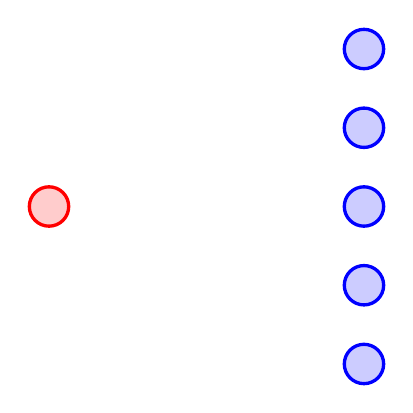
\begin{tikzpicture}[rotate=90, every node/.style={draw, very thick, circle, minimum width=0.5cm}]
                \node[red, fill=red!20!white] at (3, 0) (nd0) {};
                \foreach \i in {1,2,3,4,5} {
                    \node[blue, fill=blue!20!white] at (\i, -4) (nd1-\i) {};
                }
            \end{tikzpicture}
        \end{center}
    \end{figure}
\end{frame}

\begin{frame}{\ctitle{「代理人」}}
    \only<1> {
        \begin{figure}[h!]
            \begin{center}
                \begin{tikzpicture}[rotate=90, every node/.style={draw, very thick, circle, minimum width=0.5cm}]
                    \node[red, fill=red!20!white] at (3, 0) (nd0) {};
                    \foreach \i in {1,2,3,4,5} {
                        \node[blue, fill=blue!20!white] at (\i, -4) (nd1-\i) {};
                        \draw[->, very thick, >={Stealth}, red] (nd0) -- (nd1-\i);
                    }
                    \draw[draw=none] (nd0) -- node[red, draw=none, midway, anchor=north east]{$w$} (nd1-1);
                \end{tikzpicture}
            \end{center}
        \end{figure}
    
        注意到,建出來每一條邊都長得一模一樣
    }

    \only<2> {
        \begin{figure}[h!]
            \begin{center}
                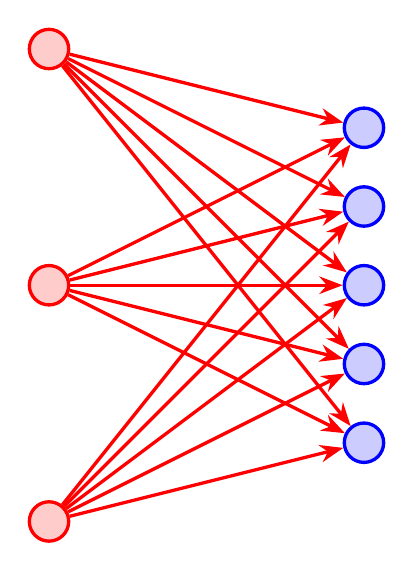
\begin{tikzpicture}[rotate=90, every node/.style={draw, very thick, circle, minimum width=0.5cm}]
                    \node[red, fill=red!20!white] at (0, 0) (nd0-1) {};
                    \node[red, fill=red!20!white] at (3, 0) (nd0-2) {};
                    \node[red, fill=red!20!white] at (6, 0) (nd0-3) {};
                    \foreach \i in {1,2,3,4,5} {
                        \node[blue, fill=blue!20!white] at (\i, -4) (nd1-\i) {};
                        \draw[->, very thick, >={Stealth}, red] (nd0-1) -- (nd1-\i);
                        \draw[->, very thick, >={Stealth}, red] (nd0-2) -- (nd1-\i);
                        \draw[->, very thick, >={Stealth}, red] (nd0-3) -- (nd1-\i);
                    }
                \end{tikzpicture}
            \end{center}
        \end{figure}
    }
    
    \only<3> {
        一次詢問建出太多邊了

        \begin{figure}[h!]
            \begin{center}
                \begin{tikzpicture}[rotate=90, every node/.style={draw, very thick, circle, minimum width=0.5cm}]
                    \node[red, fill=red!20!white] at (3, 0) (nd0) {};
                    \node[blue, fill=cyan!50!white] at (3, -3) (nd2) {};
                    \foreach \i in {1,2,3,4,5} {
                        \node[blue, fill=blue!20!white] at (\i, -4) (nd1-\i) {};
                        \draw[->, very thick, >={Stealth}, blue] (nd2) -- (nd1-\i);
                    }
                    \draw[->, very thick, >={Stealth}, red] (nd0) -- node[draw=none, midway, anchor=north east]{$w$} (nd2);
                    \draw[blue, draw=none] (nd2) -- node[draw=none, midway, anchor=north east]{$0$} (nd1-1);
                \end{tikzpicture}
            \end{center}
        \end{figure}
    
        先建一個中間點,中間點再連藍色點\\
        詢問的時候,紅色點連\yum{一條邊}到中間點
    }
    
    \only<4> {
        \begin{figure}[h!]
            \begin{center}
                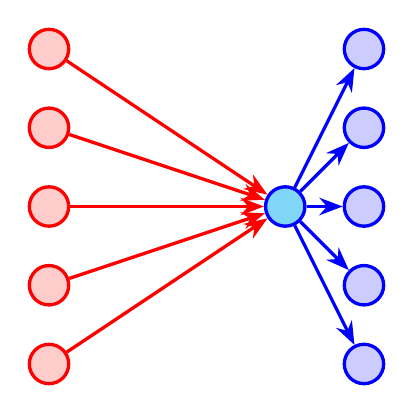
\begin{tikzpicture}[rotate=90, every node/.style={draw, very thick, circle, minimum width=0.5cm}]
                    \node[red, fill=red!20!white] at (1, 0) (nd0-1) {};
                    \node[red, fill=red!20!white] at (2, 0) (nd0-2) {};
                    \node[red, fill=red!20!white] at (3, 0) (nd0-3) {};
                    \node[red, fill=red!20!white] at (4, 0) (nd0-4) {};
                    \node[red, fill=red!20!white] at (5, 0) (nd0-5) {};
                    \node[blue, fill=cyan!50!white] at (3, -3) (nd2) {};
                    \foreach \i in {1,2,3,4,5} {
                        \node[blue, fill=blue!20!white] at (\i, -4) (nd1-\i) {};
                        \draw[->, very thick, >={Stealth}, blue] (nd2) -- (nd1-\i);
                        \draw[->, very thick, >={Stealth}, red] (nd0-\i) -- (nd2);
                    }
                \end{tikzpicture}
            \end{center}
        \end{figure}
    }

    \only<5> {
        以鬆弛的角度來說,連 $(a, b)$ 邊權 $w$,造成 $d(a) + w \ge d(b)$

        $a$ 連中間人 $c$,$d(a) + w \ge d(c)$ \\
        中間人 $c$ 連 $b_i$,$d(c) + 0 \ge d(b_i)$ \\
        $\Longrightarrow$ 實質上等同 $a$ 連 $b_i$,$d(a) + w \ge d(b_i)$
    }

\end{frame}

\begin{frame}{\ectitle}
    回到原本的問題,每次詢問要連邊的區間不一樣,每次開新的中間點的話問題沒有半點解決

    如果可以預先決定少少的中間點,每個中間點連到一個區間?\\
    如果可以預先決定一些區間,讓每個詢問都可以被這些區間拆分成少少段?

    \only<2> {
        把中間點開成\yum{線段樹}的樣子
    }
\end{frame}

\begin{frame}{\ectitle}
    \only<1> {
    \begin{figure}[h!]
        \begin{center}
            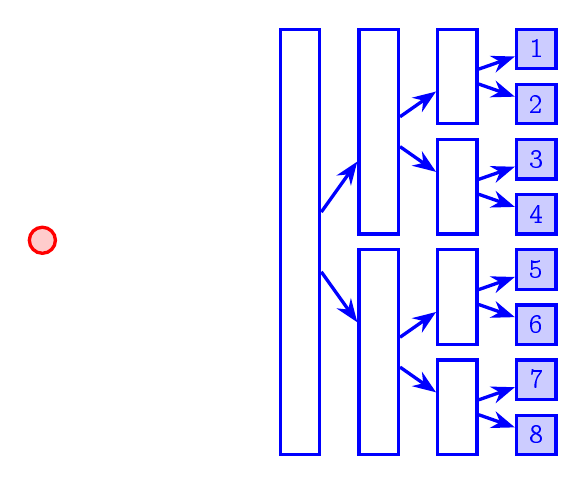
\begin{tikzpicture}[
                seg/.style={draw, very thick, rectangle, minimum width=0.5cm, anchor=north west},
                arrow/.style={->, very thick, >={Stealth}, blue},
                bluearr/.style={->, very thick, >={Stealth}, red},
                ndblue/.style={blue, fill={blue!20!white}},
                ndcyan/.style={blue, fill={cyan!50!white}},
                ndwhite/.style={blue, fill={white}},
            ]
                \node[anchor=center, draw, very thick, red, circle, fill=red!20!white] at (-3, -3.4) (nd-qry) {};

                \node[seg, ndwhite, minimum height=5.4cm] (nd-0) at (0, -0.7) {};
                \node[seg, ndwhite, minimum height=2.6cm] (nd-1) at (1, -0.7) {};
                \node[seg, ndwhite, minimum height=1.2cm] (nd-3) at (2, -0.7) {};
                \node[seg, ndblue, minimum height=0.5cm] (nd-7) at (3, -0.7) {1};
                \node[seg, ndblue, minimum height=0.5cm] (nd-8) at (3, -1.4) {2};
                \node[seg, ndwhite, minimum height=1.2cm] (nd-4) at (2, -2.1) {};
                \node[seg, ndblue, minimum height=0.5cm] (nd-9) at (3, -2.1) {3};
                \node[seg, ndblue, minimum height=0.5cm] (nd-10) at (3, -2.8) {4};
                \node[seg, ndwhite, minimum height=2.6cm] (nd-2) at (1, -3.5) {};
                \node[seg, ndwhite, minimum height=1.2cm] (nd-5) at (2, -3.5) {};
                \node[seg, ndblue, minimum height=0.5cm] (nd-11) at (3, -3.5) {5};
                \node[seg, ndblue, minimum height=0.5cm] (nd-12) at (3, -4.2) {6};
                \node[seg, ndwhite, minimum height=1.2cm] (nd-6) at (2, -4.9) {};
                \node[seg, ndblue, minimum height=0.5cm] (nd-13) at (3, -4.9) {7};
                \node[seg, ndblue, minimum height=0.5cm] (nd-14) at (3, -5.6) {8};
                \draw[arrow, blue] (nd-3) -- (nd-7);
                \draw[arrow, blue] (nd-3) -- (nd-8);
                \draw[arrow, blue] (nd-4) -- (nd-9);
                \draw[arrow, blue] (nd-4) -- (nd-10);
                \draw[arrow, blue] (nd-1) -- (nd-3);
                \draw[arrow, blue] (nd-1) -- (nd-4);
                \draw[arrow, blue] (nd-5) -- (nd-11);
                \draw[arrow, blue] (nd-5) -- (nd-12);
                \draw[arrow, blue] (nd-6) -- (nd-13);
                \draw[arrow, blue] (nd-6) -- (nd-14);
                \draw[arrow, blue] (nd-2) -- (nd-5);
                \draw[arrow, blue] (nd-2) -- (nd-6);
                \draw[arrow, blue] (nd-0) -- (nd-1);
                \draw[arrow, blue] (nd-0) -- (nd-2);
            \end{tikzpicture}
        \end{center}
    \end{figure}
    }

    \only<2> {
    \begin{figure}[h!]
        \begin{center}
            \begin{tikzpicture}[
                seg/.style={draw, very thick, rectangle, minimum width=0.5cm, anchor=north west},
                arrow/.style={->, very thick, >={Stealth}, blue},
                bluearr/.style={->, very thick, >={Stealth}, red},
                ndblue/.style={blue, fill={blue!20!white}},
                ndcyan/.style={blue, fill={cyan!50!white}},
                ndwhite/.style={blue, fill={white}},
                ndgray/.style={gray, fill={white}},
            ]
                \node[seg, ndgray, minimum height=5.4cm] (nd-0) at (0, -0.7) {};\node[seg, ndgray, minimum height=2.6cm] (nd-1) at (1, -0.7) {};\node[seg, ndgray, minimum height=1.2cm] (nd-3) at (2, -0.7) {};\node[seg, ndgray, minimum height=0.5cm] (nd-7) at (3, -0.7) {1};\node[seg, ndgray, minimum height=0.5cm] (nd-8) at (3, -1.4) {2};\node[seg, ndwhite, minimum height=1.2cm] (nd-4) at (2, -2.1) {};\node[seg, ndblue, minimum height=0.5cm] (nd-9) at (3, -2.1) {3};\node[seg, ndblue, minimum height=0.5cm] (nd-10) at (3, -2.8) {4};\node[seg, ndwhite, minimum height=2.6cm] (nd-2) at (1, -3.5) {};\node[seg, ndwhite, minimum height=1.2cm] (nd-5) at (2, -3.5) {};\node[seg, ndblue, minimum height=0.5cm] (nd-11) at (3, -3.5) {5};\node[seg, ndblue, minimum height=0.5cm] (nd-12) at (3, -4.2) {6};\node[seg, ndwhite, minimum height=1.2cm] (nd-6) at (2, -4.9) {};\node[seg, ndblue, minimum height=0.5cm] (nd-13) at (3, -4.9) {7};\node[seg, ndblue, minimum height=0.5cm] (nd-14) at (3, -5.6) {8};
                \draw[arrow, gray] (nd-3) -- (nd-7);\draw[arrow, gray] (nd-3) -- (nd-8);\draw[arrow, blue] (nd-4) -- (nd-9);\draw[arrow, blue] (nd-4) -- (nd-10);\draw[arrow, gray] (nd-1) -- (nd-3);\draw[arrow, gray] (nd-1) -- (nd-4);\draw[arrow, blue] (nd-5) -- (nd-11);\draw[arrow, blue] (nd-5) -- (nd-12);\draw[arrow, blue] (nd-6) -- (nd-13);\draw[arrow, blue] (nd-6) -- (nd-14);\draw[arrow, blue] (nd-2) -- (nd-5);\draw[arrow, blue] (nd-2) -- (nd-6);\draw[arrow, gray] (nd-0) -- (nd-1);\draw[arrow, gray] (nd-0) -- (nd-2);

                \node[anchor=center, draw, very thick, red, circle, fill=red!20!white] at (-3, -3.4) (nd-qry) {};
                \draw[arrow, red] (nd-qry) -- (nd-2);
                \draw[arrow, red] (nd-qry) -- (nd-4);
                \node[left of=nd-qry] {$[3, 8]$};
            \end{tikzpicture}
        \end{center}
    \end{figure}
    }

    \only<3> {
    \begin{figure}[h!]
        \begin{center}
            \begin{tikzpicture}[
                seg/.style={draw, very thick, rectangle, minimum width=0.5cm, anchor=north west},
                arrow/.style={->, very thick, >={Stealth}, blue},
                bluearr/.style={->, very thick, >={Stealth}, red},
                ndblue/.style={blue, fill={blue!20!white}},
                ndcyan/.style={blue, fill={cyan!50!white}},
                ndwhite/.style={blue, fill={white}},
                ndgray/.style={gray, fill={white}},
            ]
                \node[seg, ndgray, minimum height=5.4cm] (nd-0) at (0, -0.7) {};\node[seg, ndgray, minimum height=2.6cm] (nd-1) at (1, -0.7) {};\node[seg, ndgray, minimum height=1.2cm] (nd-3) at (2, -0.7) {};\node[seg, ndgray, minimum height=0.5cm] (nd-7) at (3, -0.7) {1};\node[seg, ndblue, minimum height=0.5cm] (nd-8) at (3, -1.4) {2};\node[seg, ndwhite, minimum height=1.2cm] (nd-4) at (2, -2.1) {};\node[seg, ndblue, minimum height=0.5cm] (nd-9) at (3, -2.1) {3};\node[seg, ndblue, minimum height=0.5cm] (nd-10) at (3, -2.8) {4};\node[seg, ndwhite, minimum height=2.6cm] (nd-2) at (1, -3.5) {};\node[seg, ndwhite, minimum height=1.2cm] (nd-5) at (2, -3.5) {};\node[seg, ndblue, minimum height=0.5cm] (nd-11) at (3, -3.5) {5};\node[seg, ndblue, minimum height=0.5cm] (nd-12) at (3, -4.2) {6};\node[seg, ndwhite, minimum height=1.2cm] (nd-6) at (2, -4.9) {};\node[seg, ndblue, minimum height=0.5cm] (nd-13) at (3, -4.9) {7};\node[seg, ndblue, minimum height=0.5cm] (nd-14) at (3, -5.6) {8};
                \draw[arrow, gray] (nd-3) -- (nd-7);\draw[arrow, gray] (nd-3) -- (nd-8);\draw[arrow, blue] (nd-4) -- (nd-9);\draw[arrow, blue] (nd-4) -- (nd-10);\draw[arrow, gray] (nd-1) -- (nd-3);\draw[arrow, gray] (nd-1) -- (nd-4);\draw[arrow, blue] (nd-5) -- (nd-11);\draw[arrow, blue] (nd-5) -- (nd-12);\draw[arrow, blue] (nd-6) -- (nd-13);\draw[arrow, blue] (nd-6) -- (nd-14);\draw[arrow, blue] (nd-2) -- (nd-5);\draw[arrow, blue] (nd-2) -- (nd-6);\draw[arrow, gray] (nd-0) -- (nd-1);\draw[arrow, gray] (nd-0) -- (nd-2);

                \node[anchor=center, draw, very thick, red, circle, fill=red!20!white] at (-3, -3.4) (nd-qry-1) {};
                \draw[arrow, red] (nd-qry-1) -- (nd-2);
                \draw[arrow, red] (nd-qry-1) -- (nd-4);
                \node[left of=nd-qry-1] {$[3, 8]$};
                
                \node[anchor=center, draw, very thick, red, circle, fill=red!20!white] at (-3, -1.4) (nd-qry-2) {};
                \draw[arrow, red] (nd-qry-2) -- (nd-4);
                \draw[arrow, red] (nd-qry-2) -- (nd-8);
                \node[left of=nd-qry-2] {$[2, 4]$};
                
                \node[anchor=center, draw, very thick, red, circle, fill=red!20!white] at (-3, -5.4) (nd-qry-3) {};
                \draw[arrow, red] (nd-qry-3) -- (nd-13);
                \node[left of=nd-qry-3] {$[7, 7]$};
                
            \end{tikzpicture}
        \end{center}
    \end{figure}
    }
\end{frame}

\begin{frame}{\ectitle}
    對一個線段樹節點連一條邊,等同於對區間內所有點分別連邊
    
    如果把整張圖反過來:從線段樹節點連出來,等同於從區間內所有點分別連出來
\end{frame}

\begin{frame}{\ectitle}
    預先建兩棵線段樹,一棵從根往葉子連邊,一棵從葉子往根連邊 \\
    每次詢問根據方向在對應的樹上連 $O(\log N)$ 條邊,就可以建出一樣的圖(在最短路的意義上一樣)

    單源最短路?dijkstra 就好
\end{frame}

\begin{frame}{\ectitle}
    最後建出來的圖上:
    \begin{itemize}
        \item 一棵線段樹有 $2N$ 個節點,但是兩棵線段樹葉節點可以共用,總共 $3N$ 個點
        \item 兩棵線段樹各建 $O(N)$ 條邊,之後每個詢問建 $O(\log N)$ 條邊,總共 $O(N + Q \log N)$ 條邊
    \end{itemize}
    時間複雜度 $O((N + Q \log N) \log N)$
\end{frame}

\begin{frame}{\ectitle}
    線段樹本身和我們是怎麼建圖的並\yum{沒有}關係 \\
    我們甚至可以用 sparse table 建類似的圖

    線段樹在這裡發揮的最大價值是\yum{把詢問區間拆解}成一些特別的小區間
\end{frame}



% \section{Pattern}

\begin{frame}{\ebtitle}
    \begin{quote}
        資料結構往往不會赤裸出現 \\
    
        不是「我要用這個資結砸掉這題」\\
        而是「這題需要這樣做,所以可以拿這個資結砸掉」\\
        永遠都先想怎麼做,再尋找合適的資結幫助你 \\

        -- 2024 基礎資結
    \end{quote}

    \only<2> {
        有時候,題目要你維護的東西實在是太荒謬了,你需要自己創造可以維護的東西去維護
    }
\end{frame}

\newcommand{\bigEmoji}[1]{\scalebox{2.5}{\twemoji{#1}}}
\newcommand{\mediumEmoji}[1]{\raisebox{-0.05em}{\scalebox{1.7}{\twemoji{#1}}}}
\begin{frame}{\btitle{Taxis}}
    \only<1,6-> {
        \begin{problem}[Taxis,POI 2018]
            現在有 $n$ 台計程車編號 $1\sim n$,對於第 $i$ 台計程車,給定 $s_i,c_i$,代表該台計程車的收費方式為 $s_i + d\times c_i$,其中 $d$ 為里程數。
    
            給定一個 $1\sim n$的排列,請問是否存在一個里程數 $x/y$,使得把所有計程車的編號照著收費由小到大列出\only<1-7>{恰好是這個排列}\only<8>{\yum{恰好是這個排列???}}(當收費價格一樣,順序可以任意安排),若存在的話請輸出任意一組解,否則輸出「NIE」。
    
            \only<1-6> {
                \only<4>{接著會有 $q$ 筆修改}\only<6>{\yum{接著會有 $q$ 筆修改}},每筆修改會有 $a_i,b_i$,代表交換排列在 $a_i$ 和 $b_i$ 的數字,每次交換後皆須輸出先前問題的答案。\only<6>{\yum{???}}
            }
    
            \begin{itemize}
                \item $1\le n\le 5\times10^5$。
                \item $1\le q\le 5\times10^5$。
            \end{itemize}
        \end{problem}
    }

    \only<2-5> {
        \begin{centikz}[scale=0.9]
            \draw[color=gray, ->] (-5.5, 0) -- (5.5, 0);
            \draw[color=gray, ->] (-5, -0.5) -- (-5, 5.5);
            \node[gray, anchor=north] at (5.5, 0) {\bigEmoji{sport utility vehicle}\bigEmoji{dashing away}};
            \node[gray, anchor=east]  at (-5, 5.5) {\bigEmoji{moneybag}};
            \draw[name path=line1, color=Dandelion, thick] plot[domain=-5.5:5.5] (\x,{-0.3 * \x + 2.1});
            \draw[name path=line2, color=Dandelion, thick] plot[domain=-5.5:5.5] (\x,{0.1 * \x + 3.0});
            \draw[name path=line3, color=Dandelion, thick] plot[domain=-5.5:5.5] (\x,{0.4 * \x + 2.7});
            \node[Dandelion, anchor=west] at (5.6, -0.3 * 5.5 + 2.1 + 0.1) {\underline{\mediumEmoji{taxi} $1$}};
            \node[Dandelion, anchor=west] at (5.6,  0.1 * 5.5 + 3.0 + 0.1) {\underline{\mediumEmoji{taxi} $2$}};
            \node[Dandelion, anchor=west] at (5.6,  0.4 * 5.5 + 2.7 + 0.1) {\underline{\mediumEmoji{taxi} $3$}};
            \only<3> {
                \draw[name path=vline, color=blue, dashed, very thick] (-1.5, -0.5) -- (-1.5, 5.5);
                \node[anchor=south] at (-1.5, 5.5) {$[3, 1, 2]$ \emoji{check mark button}};
                \fill [blue, right, name intersections={of=vline and line1}] (intersection-1) circle (2pt) node {$1$};
                \fill [blue, above right, name intersections={of=vline and line2}] (intersection-1) circle (2pt) node {$2$};
                \fill [blue, below right, name intersections={of=vline and line3}] (intersection-1) circle (2pt) node {$3$};
            }
            \only<4> {
                \draw[name path=vline, color=blue, dashed, very thick] (0, -0.5) -- (0, 5.5);
                \node[anchor=south] at (0, 5.5) {$[1, 3, 2]$ \emoji{check mark button}};
                \fill [blue, right, name intersections={of=vline and line1}] (intersection-1) circle (2pt) node {$1$};
                \fill [blue, above right, name intersections={of=vline and line2}] (intersection-1) circle (2pt) node {$2$};
                \fill [blue, right, name intersections={of=vline and line3}] (intersection-1) circle (2pt) node {$3$};
            }
            \only<5> {
                \node[anchor=south] at (0, 5.5) {$[2, 3, 1]$ \emoji{cross mark}};
            }
        \end{centikz}
    }
\end{frame}

\begin{frame}{\btitle{Taxis}}
    什麼時候......

    \begin{itemize}
        \item \only<2->{\emoji{vomiting_face}} \sout<2->{計程車照收費排序剛好是 $1, 2, \dots, n$}
        \only<3-> {
            \item \only<4>{\emoji{smiling face with hearts}} $1$ 號車收費 $\leq 2$ 號,而且
            \item \only<4>{\emoji{smiling face with hearts}} $2$ 號車收費 $\leq 3$ 號,而且
            \item ......
            \item \only<4>{\emoji{smiling face with hearts}} $n - 1$ 號車收費 $\leq n$ 號
        }
    \end{itemize}

    \only<4> {
        $n = 2$ 我們總會做了吧?
    }
\end{frame}

\begin{frame}{\btitle{Taxis}}
    只考慮 $i$ 號車和 $i + 1$ 號車,可以滿足「$i$ 在 $i + 1$ 前面」的距離 $d$ 是一個 $d \leq \square$ 或 $d \geq \square$ 的限制

    當每一組相鄰計程車的順序都滿足,所有車就會照順序排好
    
    \only<2> {
        維護一坨射線有沒有交集 \\
        可以用兩個 multiset 維護
    }
\end{frame}

\begin{frame}{\btitle{Taxis}}
    帶修改?

    \sout<2->{「每筆修改會有 $a_i,b_i$,代表交換排列在 $a_i$ 和 $b_i$ 的數字」}
    \only<2-> {
        \\每次都做兩個單點修改
    }

    \only<3> {
        時間複雜度:一次詢問 $O(1)$ 次 multiset 操作,總共 $O((n + q) \log n)$
    }
\end{frame}

\begin{frame}{\btitle{Grades}}
    \begin{problem}[Grades,POI 2017]
        有 $n$ 位學生編號 $1\sim n$ 以任意順序由左到右排成一列,現在你要派給這 $n$ 位學生成績,成績必須是一個介於 $1\sim n$之間的數字,且必須滿足以下條件:

        \begin{itemize}
            \item 若學生 $u$ 的編號比學生 $v$ 大,則學生 $u$ 的成績不可以小於學生 $v$。
            \item 若學生 $v$ 排在學生 $u$ 右邊一位,則學生 $v$ 的成績不可以小於學生 $u$,不然他會很傷心。
        \end{itemize}

            請問最多可以有多少不同的成績種類被派送出去?

            接著會有 $z$ 筆修改,每筆修改會有 $p_i,q_i$,代表交換排在位置 $p_i$ 和 $q_i$ 的學生編號,每次交換後皆須輸出先前問題的答案。
        \begin{itemize}
            \item $1\le n\le 10^6$。
            \item $1\le z\le 3\times10^5$。
        \end{itemize}
    \end{problem}
\end{frame}

\begin{frame}{\btitle{Grades}}
    TL;DR

    有 $n$ 個學生從左到右排成一列,編號大的、排左邊的,成績要比較高。最多能派出幾種不同的成績?

    \only<2-> {
        \only<3>{\emoji{see-no-evil monkey}} \sout<3>{$z$ 次修改,每次交換隊伍裡兩個學生的位置}
    }
\end{frame}

\begin{frame}{\btitle{Grades}}
    $n = 2$......

    \begin{itemize}
        \item $[2, 1]$:兩種
        \item $[1, 2]$:一種
    \end{itemize}
\end{frame}

\begin{frame}{\btitle{Grades}}
    有兩個人 $u < v$......

    \begin{itemize}
        \item $v$ 排 $u$ 左邊\only<2>{:$v$ 的分數本來就該比較高}
        \item $u$ 排 $v$ 左邊\only<2>{:$u, u + 1, \dots, v - 1, v$ 的分數全都要一樣!}
    \end{itemize}
\end{frame}

\begin{frame}{\btitle{Grades}}
    看兩兩相鄰學生的編號關係,獲得(最多)$n - 1$ 條限制「$u_i, u_i + 1, \dots, v_i - 1, v_i$ 的分數要一樣」

    \only<2> {
        要怎麼詢問「最多能派出幾種不同的成績」?
    }

    \only<3> {
        每條限制都是「$u_i + 1, \dots, v_i - 1, v_i$ 的分數都固定了,只有 $u_i$ 的分數可以自由決定」\\
        最後數數看有幾個人的分數可以自由決定
    }

    \only<4> {
        每條限制都是「\yum{$u_i + 1, \dots, v_i - 1, v_i$} 的分數都固定了,只有 $u_i$ 的分數可以自由決定」\\
        最後數數看有幾個人的分數可以自由決定

        \yum{區間加值($\pm 1$),數數看全域有幾個 $0$}
    }
\end{frame}

\begin{frame}{\btitle{Grades}}
    帶修改(交換兩人位置)?
    
    依然可以是兩次單點修改
\end{frame}

\begin{frame}{\btitle{Grades}}
    區間加值、單點修改、數全域有幾個 $0$

    拿你最喜歡的資料結構砸掉 \\
    時間複雜度 $O((n + z) \log n)$
\end{frame}

\begin{frame}{\ebtitle}
    我們是怎麼做完前面兩題的?

    \begin{itemize}
        \item 題目要維護的東西難以維護(整個排列的長相)
        \item 找到小小的特徵點,用小特徵湊出題目要的條件(排列中相鄰元素關係)
        \item 小特徵足夠單純可以維護(multiset、線段樹)
    \end{itemize}
\end{frame}

\begin{frame}{\btitle{Seats}}
    \begin{problem}[Seats,IOI 2018]
        (完整敘述請見講義)\\

        有 $H \times W$ 個位子排成一個矩形,還有 $HW$ 位選手每人分別佔一個位置。有幾個\yum{矩形},使得矩形區域內坐的選手的編號恰好是 $0$ 開始的連續數字?\\

        支援 $Q$ 次修改,每次交換兩位選手的位置,每次交換完輸出以上問題的答案。\\

        \begin{itemize}
            \item $1 \le H \times W \le 10^6$
            \item $1 \le Q \le 5 \times 10^4$
        \end{itemize}
    \end{problem}
\end{frame}

\begin{frame}{\btitle{Seats}}
    \todo 插圖
\end{frame}

\begin{frame}{\btitle{Seats}}
    \begin{problem}[Seats,IOI 2018]
        Subtasks

        \begin{itemize}
            \item (5) $HW \le 100$,$Q \le 5000$
            \item (6) $HW \le 10^4$,$Q \le 5000$
            \item (20) $H \le 1000$,$W \le 1000$,$Q \le 5000$
            \item (6) $Q \le 5000$,對於每次交換 $|a - b| \le 10^4$
            \item (33) $H = 1$
            \item (30) 無額外限制
        \end{itemize}
    \end{problem}
    
    拿零分還可以金牌的難題!?
\end{frame}

\begin{frame}{\btitle{Seats}}
    選手一個一個坐進去,檢查他們是不是坐成矩形的樣子

    躲不開的障礙:\\
    要怎麼檢查一個矩形範圍是不是好的?\\
    要怎麼檢查 $0, \dots, rc - 1$ 的範圍是不是好的?
\end{frame}

\begin{frame}{\btitle{Seats}}
    \begin{problem}[Seats,IOI 2018]
        Subtasks

        \begin{itemize}
            \item (5) $HW \le 100$,$Q \le 5000$
            \item (6) $HW \le 10^4$,$Q \le 5000$
            \item (20) $H \le 1000$,$W \le 1000$,$Q \le 5000$
            \item (6) $Q \le 5000$,對於每次交換 $|a - b| \le 10^4$
            \item \tikzoverlay{nd0}{}\yum{(33) $H = 1$}
            \item (30) 無額外限制
        \end{itemize}
    \end{problem}

    二維太荒謬了,先想辦法搞定一維

    \begin{tikzpicture}[remember picture, overlay]
        \node[draw=WildStrawberry, very thick, left=0.1cm of nd0, anchor=base west] {\phantom{\yum{(33) $H = 1$}}};
    \end{tikzpicture}
\end{frame}

\begin{frame}{\btitle{Seats}}
    選手一個一個坐進去,檢查他們是不是坐成連續區間的樣子

    躲不開的障礙:\\
    要怎麼檢查一個區間是不是好的?\\
    要怎麼檢查 $0, \dots, rc - 1$ 的範圍是不是好的?
\end{frame}

\begin{frame}{\btitle{Seats}}
    \todo
\end{frame}

\begin{frame}{\btitle{Seats}}
    把 $0, \dots, rc - 1$ 塗黑色,其他格子和界外留白。他們剛好在一個連續區間的\yum{充要條件}是......

    \only<2> {
        對於每一組相鄰的格子,\yum{恰好有兩組是一黑一白} \\
    }
\end{frame}

\begin{frame}{\btitle{Seats}}
    \todo
\end{frame}

\begin{frame}{\btitle{Seats}}
    把 $0, 1, \dots, HW - 1$ 一個一個塗黑,每個時間點檢查是不是恰好兩組格子是一黑一白
\end{frame}

\begin{frame}{\btitle{Seats}}
    對於每一組相鄰的格子,他們在\only<1>{哪些時間是一黑一白?}\only<2->{\strong{某個連續的時間區間}是一黑一白}

    \only<2> {
        拿出你最喜歡的資料結構,維護每個時間點一黑一白的格子有幾組,數數看全域有幾個 $2$
    }

    \only<3> {
        拿出你最喜歡的資料結構,維護每個時間點一黑一白的格子有幾組,\yum{數數看全域有幾個 $2$???}
    }

    \only<4> {
        只要有格子是黑的,一黑一白的格子就至少有兩組

        拿出你最喜歡的資料結構,維護每個時間點一黑一白的格子有幾組,\strong{檢查全域最小值是不是 $2$、數數看最小值有幾個}
    }
\end{frame}

\begin{frame}{\btitle{Seats}}
    修改?還是可以兩次單點修改

    時間複雜度:$O((W + Q) \log W)$
\end{frame}

\begin{frame}{\btitle{Seats}}
    \begin{problem}[Seats,IOI 2018]
        Subtasks

        \begin{itemize}
            \item (5) $HW \le 100$,$Q \le 5000$
            \item (6) $HW \le 10^4$,$Q \le 5000$
            \item (20) $H \le 1000$,$W \le 1000$,$Q \le 5000$
            \item (6) $Q \le 5000$,對於每次交換 $|a - b| \le 10^4$
            \item (33) $H = 1$
            \item \tikzoverlay{nd0}{}\yum{(30) 無額外限制}
        \end{itemize}
    \end{problem}

    \begin{tikzpicture}[remember picture, overlay]
        \node[draw=WildStrawberry, very thick, left=0.1cm of nd0, anchor=base west] {\phantom{\yum{(30) 無額外限制}}};
    \end{tikzpicture}
\end{frame}

\begin{frame}{\btitle{Seats}}
    \todo
\end{frame}

\begin{frame}{\btitle{Seats}}
    把 $0, \dots, rc - 1$ 塗黑色,其他格子和界外留白。他們剛好形成一個矩形的\yum{充要條件}是......

    \only<2> {
        對於每一塊 $2 \times 2$ 相鄰的格子,
        \begin{itemize}
            \item 恰好四塊是一黑三白
        \end{itemize}
    }
\end{frame}

\begin{frame}{\btitle{Seats}}
    \todo:甜甜圈
\end{frame}

\begin{frame}{\btitle{Seats}}
    把 $0, \dots, rc - 1$ 塗黑色,其他格子和界外留白。他們剛好形成一個矩形的\yum{充要條件}是......

    對於每一塊 $2 \times 2$ 相鄰的格子,
    \begin{itemize}
        \item 恰好 $4$ 塊是一黑三白
        \item \strong{沒有任何一塊是三黑一白}
    \end{itemize}
\end{frame}

\begin{frame}{\btitle{Seats}}
    \todo
\end{frame}

\begin{frame}{\btitle{Seats}}
    對於每一組 $2 \times 2$ 的格子,他們在\only<1>{哪些時間是一黑三白、或是三黑一白?}\only<2->{\strong{某個連續的時間區間}是一黑三白、或是三黑一白}

    \only<2> {
        只要有格子是黑的,一黑三白的格子就至少有 $4$ 組

        拿出你最喜歡的資料結構,維護每個時間點一黑三白、三黑一白的格子有幾組,\strong{檢查全域最小值是不是 $4$、數數看最小值有幾個}
    }
\end{frame}

\begin{frame}{\btitle{Seats}}
    修改?還是可以兩次單點修改

    \only<1> {
        時間複雜度:$O((HW + Q) \log HW)$ \\
        (多花點力氣 $O(HW + Q \log HW)$)
    }

    \only<2> {
        時間複雜度:$O(HW + \yum{16}Q \log HW)$ \\
        常數巨大!
    }
\end{frame}

\begin{frame}{\btitle{好的連續子序列}}
    \begin{problem}[好的連續子序列,台大演算法設計與分析(ADA)作業]
        給定一個 $1, 2, \dots, N$ 的排列,試求有多少子區間 $[l,r]$,滿足該子區間是一個連續正整數的排列?

        \begin{itemize}
            \item $1\le N \le 5\times10^5$
        \end{itemize}
    \end{problem}

    在 Codeforces 526F 有可以傳的 Judge
\end{frame}

\begin{frame}{\btitle{好的連續子序列}}
    跟一維的 Seats 比起來,少了修改,多了不是 $1$ 開頭的區間也要數數看

    \only<2-> {
        \begin{itemize}
            \item 用 Seats 作法找出 $1$ 開頭的好區間有幾個
            \item 把 $1$ 拿掉(讓他永遠是白色),找出 $2$ 開頭的好區間有幾個
            \item ......
            \item 把 $1, 2, \dots, N - 1$ 拿掉(讓他們永遠是白色),找出 $N$ 開頭的好區間有幾個
        \end{itemize}
    }

    \only<3> {
        題目沒叫你修改,但是你自己把「枚舉排列的開頭」當成 $N$ 次修改
    }
\end{frame}

\begin{frame}{\btitle{好的連續子序列}}
    \only<1> {
        時間複雜度:$O(N \log N)$
    }

    \only<2> {
        時間複雜度:\yum{至少 $O(4N \log N)$}

        常數巨大!我在 NEOJ 吃 TLE
    }
\end{frame}

\begin{frame}{\btitle{好的連續子序列:番外}}
    本題官方作法是分治,也有其他使用大資料結構但可以時限內通過的作法

    你能想到幾種不同的作法?
\end{frame}

\begin{frame}{\btitle{好的連續子序列:番外}}
    關鍵觀察:好區間 $\iff r - l = \max_{l \leq i \leq r}(a_i) - \min_{l \leq i \leq r}(a_i)$

    \only<2> {
        分治作法($O(N \log N)$)
    
        \begin{itemize}
            \item 序列切兩半,數跨兩邊的好的子序列
            \begin{itemize}
                \item 分四種情況:最大值和最小值分別在左半邊還是右半邊
                \item 時間複雜度 $O(N)$
            \end{itemize}
            \item 兩邊遞迴分治
        \end{itemize}
    }
    \only<3> {
        資料結構作法($O(N \log N)$)
    
        \begin{itemize}
            \item 掃描線枚舉區間右界,用資結維護每個左界對應到的 $\left(\left(\max - \min\right) - \left(r - l\right)\right)$
            \begin{itemize}
                \item $\max, \min$ 都可以單調隊列區間加值
                \item 數數看有幾個 $0$
                \item 這坨總是 $\geq 0$,可以數最小值個數
            \end{itemize}
        \end{itemize}
    }
\end{frame}

\begin{frame}{\ebtitle}
    \begin{itemize}
        \item 題目要維護的東西難以維護
        \item 找到小小的特徵點,用小特徵湊出題目要的條件
        \item 小特徵足夠單純可以維護
    \end{itemize}

    資結不是重點,重點是發現精妙的轉換和觀察
\end{frame}

% \section{線段樹的暴力與懶人標記}

\begin{frame}{\ebtitle}
    Change my mind:均攤分析就是玄學
\end{frame}

\begin{frame}{\btitle{區間開根號}}
    \begin{problem}[帶修改區間和,Zerojudge c652]
        給你一段 $N$ 個正整數的序列 $a_1,\cdots,a_N$,請你執行 $Q$ 筆操作。

        \begin{itemize}
            \item $0\;l\;r$:代表詢問 $[l,r]$ 區間的和。
            \item $1\;l\;r$:代表將 $[l,r]$ 區間的每個數字 $a_i$ 改成 $\lfloor{\sqrt{a_i}}\rfloor$。
        \end{itemize}

        \begin{itemize}
            \item $1\le N,Q\le 3\times 10^5$。
            \item $1\le a_i\le 10^{12}$。
        \end{itemize}
    \end{problem}
\end{frame}

\begin{frame}{\btitle{區間開根號}}
    如果想在線段樹維護區間和 \\
    區間開根號的時候區間和會如何變化?

    \only<2> {
        我也不知道 \emoji{sob}

        區間開根號沒有\strong{可預測性},不能打懶人標記
    }
\end{frame}

\begin{frame}{\btitle{區間開根號}}
    觀察:一個數字被開 $\log \log C$ 次根號之後就不會再動了,永遠都會是 $1$

    \only<2> {
        \begin{itemize}
            \item 如果區間內有人不是 $1$,暴力往下修改
            \item 如果區間內所有人都是 $1$,什麼事都不需要做
        \end{itemize}

        一個數字只會被暴力改 $\log \log C$ 次,每次 $O(\log N)$ 時間 \\
        總時間複雜度 $O(Q \log N + N \log N \log\log C)$
    }
\end{frame}

\begin{frame}{\btitle{區間開根號.其二}}
    \begin{problem}[帶修改區間和 Ex.,波路自編題]
        給你一段 $N$ 個正整數的序列 $a_1,\cdots,a_N$,請你執行 $Q$ 筆操作。

        \begin{itemize}
            \item \yum{$1\;l\;r\;c$:代表將 $[l,r]$ 區間的每個數字 $a_i$ 加上 $c$。}
            \item $2\;l\;r$:代表將 $[l,r]$ 區間的每個數字 $a_i$ 改成 $\lfloor{\sqrt{a_i}}\rfloor$。
            \item $3\;l\;r$:代表詢問 $[l,r]$ 區間的和。
        \end{itemize}

        \begin{itemize}
            \item $1\le N,Q\le 10^5$。
            \item $0\le a_i,c\le 10^9$。
        \end{itemize}
    \end{problem}
\end{frame}

\begin{frame}{\btitle{區間開根號.其二}}
    開完根號再加值,一個數字只會被暴力改......$O(Q)$ 次(???)

    剛剛的作法壞掉了
\end{frame}

\begin{frame}{\btitle{區間開根號.其二}}
    \only<1> {
        觀察:區間全距被開幾次根號之後就幾乎不動了
    }

    \only<2> {
        觀察:區間全距被開 \yum{$O(\log\log C)$} 次根號之後就會一直是 \yum{$0$ 或 $1$}

        對全距是 $1$ 的區間開根號可以打懶人標記嗎?\\
        可以,多紀錄最小值和最小值個數就知道區間裡有哪些數字

        線段樹修改時,只要全距還不是 $1$ 就暴力往下修改
    }
\end{frame}

\begin{frame}{\btitle{區間開根號.其二}}
    一開始,每個節點的全距都是 $O(C)$,暴力往下次數 $O(N \log\log C)$

    每次區間加值讓 $O(\log N)$ 個節點的全距增加 $O(C)$,暴力往下次數增加 $O(\log N \log\log C)$

    總時間複雜度 $O(Q \log N + N \log\log C + Q \log N \log\log C)$
\end{frame}

\begin{frame}[fragile]{\ebtitle}
    \begin{minted}[linenos=false]{cpp}
        void modify(int node, int l, int r, int ql, int qr) {
            if(l >= ql && r <= qr) {
                give_tag(node); return;
            }
            push(node);
            int m = (l + r) / 2;
            if(ql <= m) modify(L(node), l, m, ql, qr);
            if(qr > m)  modify(R(node), m + 1, r, ql, qr);
            pull(node);
        }
    \end{minted}
\end{frame}

\begin{frame}[fragile]{\ebtitle}
    \begin{minted}[linenos=false]{cpp}
        void modify(int node, int l, int r, int ql, int qr) {
            if(l >= ql && r <= qr && 全距 <= 1) {
                give_tag(node); return;
            }
            push(node);
            int m = (l + r) / 2;
            if(ql <= m) modify(L(node), l, m, ql, qr);
            if(qr > m)  modify(R(node), m + 1, r, ql, qr);
            pull(node);
        }
    \end{minted}
\end{frame}

\begin{frame}[fragile]{\ebtitle}
    \begin{minted}[linenos=false]{cpp}
        void modify(int node, int l, int r, int ql, int qr) {
            if(tag_condition(node)) {
                give_tag(node); return;
            }
            push(node);
            int m = (l + r) / 2;
            if(ql <= m) modify(L(node), l, m, ql, qr);
            if(qr > m)  modify(R(node), m + 1, r, ql, qr);
            pull(node);
        }
    \end{minted}
\end{frame}

\begin{frame}{\ebtitle}
    也許......\mintinline{cpp}|tag_condition| 還可以是......?
\end{frame}

\begin{frame}{\btitle{Segment Tree Beats}}
    \begin{problem}[Gorgeous Sequence,HDU 5306]
        $T$ 筆測資,每筆測資給你一段 $N$ 個整數的序列 $a_1,\cdots,a_N$,請你執行 $Q$ 筆操作。

        \begin{itemize}
            \item $0\;l\;r\;t$:代表將 $[l,r]$ 區間的每個數字 $a_i$ 改成 $\min(a_i,t)$。
            \item $1\;l\;r$:代表詢問 $[l,r]$ 區間的最大值。
            \item $2\;l\;r$:代表詢問 $[l,r]$ 區間的和。
        \end{itemize}
        
        \begin{itemize}
            \item $1\le T\le 100$。
            \item $1\le \sum N,\sum Q\le 10^6$。
            \item $0\le a_i,t< 2^{31}$。
        \end{itemize}
    \end{problem}

    區間取 min 對區間和同樣不能預測,不能直接打懶人標記
\end{frame}

\begin{frame}{\btitle{Segment Tree Beats}}
    每個節點維護\yum{區間嚴格次大值}\only<2->{ \brilliance{brilliant} }和最大值個數

    \only<2-> {
        \begin{itemize}
            \item 如果 $t \leq$ 次大值,暴力往下修改
            \item 如果 $t >$ 次大值,等同於把所有最大值都改成 $t$,可以打懶人標記
        \end{itemize}

        時間複雜度:$O((N + Q) \log N)$\only<3>{???\\}
        \only<3>{憑什麼這麼快?}
    }
\end{frame}

\begin{frame}{\btitle{Segment Tree Beats}}
    考慮每個節點的數字種類數 \\
    每次往下暴力修改,額外花 $O(1)$ 時間,區間內的數字一定會少至少一種

    比一般線段樹多付出的時間 \\
    最多是每個節點暴力往下修改的總次數 \\
    也就是 $O(N \log N)$

    \only<2> {
        總時間複雜度 $O((N + Q) \log N)$
    }
\end{frame}

\begin{frame}{\btitle{Segment Tree Beats.其二}}
    \begin{problem}
        給你一段 $N$ 個整數的序列 $a_1,\cdots,a_N$,請你執行 $Q$ 筆操作。

        \begin{itemize}
            \item $0\;l\;r\;t$:代表將 $[l,r]$ 區間的每個數字 $a_i$ 改成 $\min(a_i,t)$。
            \item \yum{$1\;l\;r\;c$:代表將 $[l,r]$ 區間的每個數字加上 $c$。}
            \item $2\;l\;r$:代表詢問 $[l,r]$ 區間的最大值。
            \item $3\;l\;r$:代表詢問 $[l,r]$ 區間的和。
        \end{itemize}

        \begin{itemize}
            \item $1\le N,Q\le 3\times 10^5$。
            \item $-10^6\le c,a_i,t\le 10^6$。
        \end{itemize}
    \end{problem}
\end{frame}

\begin{frame}{\btitle{Segment Tree Beats.其二}}
    嘗試跟前一題用一樣的作法

    區間加值後,節點的數字種類數會變多......\\
    \only<2->{$O(\text{區間長度})$}

    \only<2->{沿用相同的證明想法,暴力修改的次數最多是......\\}
    \only<3->{$O(NQ)$?}

    \only<4>{
        換一種證明思路,可以證明總複雜度是 $O((N + Q) \log^2 N)$ 的
    }
\end{frame}

\begin{frame}{\btitle{Segment Tree Beats.其二}}
    序列 $[5, 4, 8, 7, 1, 6, 3, 2]$

    \begin{centikz}[
        seg/.style={draw, very thick, rectangle, minimum height=0.6cm, anchor=north west},
        seq/.style={rectangle, minimum height=0.5cm, anchor=north west, minimum width=0.6cm, black},
        ndblue/.style={blue, fill={blue!20!white}},
        ndred/.style={red, fill={red!20!white}},
        ndgreen/.style={ForestGreen, fill={ForestGreen!20!white}},
        ndgray/.style={black, fill={white}},
    ]
        \node[seg, ndgray, minimum width=6.20cm] (nd-0) at (0.80, -0.00) {\color{black}8};\node[seg, ndgray, minimum width=3.00cm] (nd-1) at (0.80, -0.80) {\color{black}};\node[seg, ndgray, minimum width=1.40cm] (nd-3) at (0.80, -1.60) {\color{black}5};\node[seg, ndgray, minimum width=0.60cm] (nd-7) at (0.80, -2.40) {\color{black}};\node[seg, ndgray, minimum width=0.60cm] (nd-8) at (1.60, -2.40) {\color{black}4};\node[seg, ndgray, minimum width=1.40cm] (nd-4) at (2.40, -1.60) {\color{black}};\node[seg, ndgray, minimum width=0.60cm] (nd-9) at (2.40, -2.40) {\color{black}};\node[seg, ndgray, minimum width=0.60cm] (nd-10) at (3.20, -2.40) {\color{black}7};\node[seg, ndgray, minimum width=3.00cm] (nd-2) at (4.00, -0.80) {\color{black}6};\node[seg, ndgray, minimum width=1.40cm] (nd-5) at (4.00, -1.60) {\color{black}};\node[seg, ndgray, minimum width=0.60cm] (nd-11) at (4.00, -2.40) {\color{black}1};\node[seg, ndgray, minimum width=0.60cm] (nd-12) at (4.80, -2.40) {\color{black}};\node[seg, ndgray, minimum width=1.40cm] (nd-6) at (5.60, -1.60) {\color{black}3};\node[seg, ndgray, minimum width=0.60cm] (nd-13) at (5.60, -2.40) {\color{black}};\node[seg, ndgray, minimum width=0.60cm] (nd-14) at (6.40, -2.40) {\color{black}2};\node[seq] at (0.8, -3.2) {5};\node[seq] at (1.6, -3.2) {4};\node[seq] at (2.4, -3.2) {8};\node[seq] at (3.2, -3.2) {7};\node[seq] at (4.0, -3.2) {1};\node[seq] at (4.8, -3.2) {6};\node[seq] at (5.6, -3.2) {3};\node[seq] at (6.4, -3.2) {2}; \draw[black, thick] (nd-7) -- (nd-3);\draw[black, thick] (nd-8) -- (nd-3);\draw[black, thick] (nd-9) -- (nd-4);\draw[black, thick] (nd-10) -- (nd-4);\draw[black, thick] (nd-3) -- (nd-1);\draw[black, thick] (nd-4) -- (nd-1);\draw[black, thick] (nd-11) -- (nd-5);\draw[black, thick] (nd-12) -- (nd-5);\draw[black, thick] (nd-13) -- (nd-6);\draw[black, thick] (nd-14) -- (nd-6);\draw[black, thick] (nd-5) -- (nd-2);\draw[black, thick] (nd-6) -- (nd-2);\draw[black, thick] (nd-1) -- (nd-0);\draw[black, thick] (nd-2) -- (nd-0);
    \end{centikz}
\end{frame}

\begin{frame}{\btitle{Segment Tree Beats.其二}}
    $[1, 6]$ 區間對 $5$ 取 min

    \begin{centikz}[
        seg/.style={draw, very thick, rectangle, minimum height=0.6cm, anchor=north west},
        seq/.style={rectangle, minimum height=0.5cm, anchor=north west, minimum width=0.6cm, black},
        ndblue/.style={blue, fill={blue!20!white}},
        ndred/.style={red, fill={red!20!white}},
        ndgreen/.style={ForestGreen, fill={ForestGreen!20!white}},
        ndgray/.style={black, fill={white}},
    ]
        \node[seg, ndgray, minimum width=6.20cm] (nd-0) at (0.80, -0.00) {\color{black}5};\node[seg, ndgray, minimum width=3.00cm] (nd-1) at (0.80, -0.80) {\color{black}};\node[seg, ndgray, minimum width=1.40cm] (nd-3) at (0.80, -1.60) {\color{black}};\node[seg, ndgray, minimum width=0.60cm] (nd-7) at (0.80, -2.40) {\color{black}};\node[seg, ndgray, minimum width=0.60cm] (nd-8) at (1.60, -2.40) {\color{black}4};\node[seg, ndgray, minimum width=1.40cm] (nd-4) at (2.40, -1.60) {\color{black}};\node[seg, ndgray, minimum width=0.60cm] (nd-9) at (2.40, -2.40) {\color{black}};\node[seg, ndgray, minimum width=0.60cm] (nd-10) at (3.20, -2.40) {\color{black}};\node[seg, ndgray, minimum width=3.00cm] (nd-2) at (4.00, -0.80) {\color{black}};\node[seg, ndgray, minimum width=1.40cm] (nd-5) at (4.00, -1.60) {\color{black}};\node[seg, ndgray, minimum width=0.60cm] (nd-11) at (4.00, -2.40) {\color{black}1};\node[seg, ndgray, minimum width=0.60cm] (nd-12) at (4.80, -2.40) {\color{black}};\node[seg, ndgray, minimum width=1.40cm] (nd-6) at (5.60, -1.60) {\color{black}3};\node[seg, ndgray, minimum width=0.60cm] (nd-13) at (5.60, -2.40) {\color{black}};\node[seg, ndgray, minimum width=0.60cm] (nd-14) at (6.40, -2.40) {\color{black}2};\node[seq] at (0.8, -3.2) {5};\node[seq] at (1.6, -3.2) {4};\node[seq] at (2.4, -3.2) {5};\node[seq] at (3.2, -3.2) {5};\node[seq] at (4.0, -3.2) {1};\node[seq] at (4.8, -3.2) {5};\node[seq] at (5.6, -3.2) {3};\node[seq] at (6.4, -3.2) {2}; \draw[black, thick] (nd-7) -- (nd-3);\draw[black, thick] (nd-8) -- (nd-3);\draw[black, thick] (nd-9) -- (nd-4);\draw[black, thick] (nd-10) -- (nd-4);\draw[black, thick] (nd-3) -- (nd-1);\draw[black, thick] (nd-4) -- (nd-1);\draw[black, thick] (nd-11) -- (nd-5);\draw[black, thick] (nd-12) -- (nd-5);\draw[black, thick] (nd-13) -- (nd-6);\draw[black, thick] (nd-14) -- (nd-6);\draw[black, thick] (nd-5) -- (nd-2);\draw[black, thick] (nd-6) -- (nd-2);\draw[black, thick] (nd-1) -- (nd-0);\draw[black, thick] (nd-2) -- (nd-0);
    \end{centikz}
\end{frame}

\begin{frame}{\btitle{Segment Tree Beats.其二}}
    標記變不一樣的節點

    \begin{centikz}[
        seg/.style={draw, very thick, rectangle, minimum height=0.6cm, anchor=north west},
        seq/.style={rectangle, minimum height=0.5cm, anchor=north west, minimum width=0.6cm, black},
        ndblue/.style={blue, fill={blue!20!white}},
        ndred/.style={red, fill={red!20!white}},
        ndgreen/.style={ForestGreen, fill={ForestGreen!20!white}},
        ndgray/.style={black, fill={white}},
    ]
        \node[seg, ndblue, minimum width=6.20cm] (nd-0) at (0.80, -0.00) {\color{blue}$8 \rightarrow 5$};\node[seg, ndgray, minimum width=3.00cm] (nd-1) at (0.80, -0.80) {\color{black}};\node[seg, ndblue, minimum width=1.40cm] (nd-3) at (0.80, -1.60) {\color{blue}$\xcancel{5}$};\node[seg, ndgray, minimum width=0.60cm] (nd-7) at (0.80, -2.40) {\color{black}};\node[seg, ndgray, minimum width=0.60cm] (nd-8) at (1.60, -2.40) {\color{black}4};\node[seg, ndgray, minimum width=1.40cm] (nd-4) at (2.40, -1.60) {\color{black}};\node[seg, ndgray, minimum width=0.60cm] (nd-9) at (2.40, -2.40) {\color{black}};\node[seg, ndblue, minimum width=0.60cm] (nd-10) at (3.20, -2.40) {\color{blue}$\xcancel{7}$};\node[seg, ndblue, minimum width=3.00cm] (nd-2) at (4.00, -0.80) {\color{blue}$\xcancel{6}$};\node[seg, ndgray, minimum width=1.40cm] (nd-5) at (4.00, -1.60) {\color{black}};\node[seg, ndgray, minimum width=0.60cm] (nd-11) at (4.00, -2.40) {\color{black}1};\node[seg, ndgray, minimum width=0.60cm] (nd-12) at (4.80, -2.40) {\color{black}};\node[seg, ndgray, minimum width=1.40cm] (nd-6) at (5.60, -1.60) {\color{black}3};\node[seg, ndgray, minimum width=0.60cm] (nd-13) at (5.60, -2.40) {\color{black}};\node[seg, ndgray, minimum width=0.60cm] (nd-14) at (6.40, -2.40) {\color{black}2};\node[seq] at (0.8, -3.2) {5};\node[seq] at (1.6, -3.2) {4};\node[seq] at (2.4, -3.2) {5};\node[seq] at (3.2, -3.2) {5};\node[seq] at (4.0, -3.2) {1};\node[seq] at (4.8, -3.2) {5};\node[seq] at (5.6, -3.2) {3};\node[seq] at (6.4, -3.2) {2}; \draw[black, thick] (nd-7) -- (nd-3);\draw[black, thick] (nd-8) -- (nd-3);\draw[black, thick] (nd-9) -- (nd-4);\draw[black, thick] (nd-10) -- (nd-4);\draw[black, thick] (nd-3) -- (nd-1);\draw[black, thick] (nd-4) -- (nd-1);\draw[black, thick] (nd-11) -- (nd-5);\draw[black, thick] (nd-12) -- (nd-5);\draw[black, thick] (nd-13) -- (nd-6);\draw[black, thick] (nd-14) -- (nd-6);\draw[black, thick] (nd-5) -- (nd-2);\draw[black, thick] (nd-6) -- (nd-2);\draw[black, thick] (nd-1) -- (nd-0);\draw[black, thick] (nd-2) -- (nd-0);
    \end{centikz}
\end{frame}

\begin{frame}{\btitle{Segment Tree Beats.其二}}
    修改過程中原本就會遞迴到的節點、和暴力往下修改的節點

    \begin{centikz}[
        seg/.style={draw, very thick, rectangle, minimum height=0.6cm, anchor=north west},
        seq/.style={rectangle, minimum height=0.5cm, anchor=north west, minimum width=0.6cm, black},
        ndblue/.style={blue, fill={blue!20!white}},
        ndred/.style={red, fill={red!20!white}},
        ndgreen/.style={ForestGreen, fill={ForestGreen!20!white}},
        ndgray/.style={black, fill={white}},
    ]
        \node[seg, ndgreen, minimum width=6.20cm] (nd-0) at (0.80, -0.00) {\color{ForestGreen}$8 \rightarrow 5$};\node[seg, ndgreen, minimum width=3.00cm] (nd-1) at (0.80, -0.80) {\color{ForestGreen}};\node[seg, ndred, minimum width=1.40cm] (nd-3) at (0.80, -1.60) {\color{red}$\xcancel{5}$};\node[seg, ndgray, minimum width=0.60cm] (nd-7) at (0.80, -2.40) {\color{black}};\node[seg, ndgray, minimum width=0.60cm] (nd-8) at (1.60, -2.40) {\color{black}4};\node[seg, ndred, minimum width=1.40cm] (nd-4) at (2.40, -1.60) {\color{red}};\node[seg, ndred, minimum width=0.60cm] (nd-9) at (2.40, -2.40) {\color{red}};\node[seg, ndred, minimum width=0.60cm] (nd-10) at (3.20, -2.40) {\color{red}$\xcancel{7}$};\node[seg, ndgreen, minimum width=3.00cm] (nd-2) at (4.00, -0.80) {\color{ForestGreen}$\xcancel{6}$};\node[seg, ndgreen, minimum width=1.40cm] (nd-5) at (4.00, -1.60) {\color{ForestGreen}};\node[seg, ndgray, minimum width=0.60cm] (nd-11) at (4.00, -2.40) {\color{black}1};\node[seg, ndgray, minimum width=0.60cm] (nd-12) at (4.80, -2.40) {\color{black}};\node[seg, ndgray, minimum width=1.40cm] (nd-6) at (5.60, -1.60) {\color{black}3};\node[seg, ndgray, minimum width=0.60cm] (nd-13) at (5.60, -2.40) {\color{black}};\node[seg, ndgray, minimum width=0.60cm] (nd-14) at (6.40, -2.40) {\color{black}2};\node[seq] at (0.8, -3.2) {5};\node[seq] at (1.6, -3.2) {4};\node[seq] at (2.4, -3.2) {5};\node[seq] at (3.2, -3.2) {5};\node[seq] at (4.0, -3.2) {1};\node[seq] at (4.8, -3.2) {5};\node[seq] at (5.6, -3.2) {3};\node[seq] at (6.4, -3.2) {2}; \draw[black, thick] (nd-7) -- (nd-3);\draw[black, thick] (nd-8) -- (nd-3);\draw[black, thick] (nd-9) -- (nd-4);\draw[black, thick] (nd-10) -- (nd-4);\draw[black, thick] (nd-3) -- (nd-1);\draw[black, thick] (nd-4) -- (nd-1);\draw[black, thick] (nd-11) -- (nd-5);\draw[black, thick] (nd-12) -- (nd-5);\draw[black, thick] (nd-13) -- (nd-6);\draw[black, thick] (nd-14) -- (nd-6);\draw[black, thick] (nd-5) -- (nd-2);\draw[black, thick] (nd-6) -- (nd-2);\draw[black, thick] (nd-1) -- (nd-0);\draw[black, thick] (nd-2) -- (nd-0);
    \end{centikz}
\end{frame}

\begin{frame}{\btitle{Segment Tree Beats.其二}}
    「$t \leq$ 區間次小值時,往下暴力」\\
    實際上等同往下 DFS 移除子樹內 $\geq t$ 的標記

    \only<2> {
        移除一個標記要花 $O(\text{樹高}) = O(\log N)$ 時間

        一開始最多有 $N$ 個標記 \\
        什麼時候標記會變多?
    }
\end{frame}

\begin{frame}{\btitle{Segment Tree Beats.其二}}
    在線段樹上區間操作的時候,可以把節點分成四種

    \begin{enumerate}[A]
        \item 被操作區間完全包含
        \item 跟操作區間部份重疊
        \item 跟操作區間不重疊,但是 B 的子節點
        \item 跟操作區間不重疊的其他節點
    \end{enumerate}

    \begin{centikz}[
        seg/.style={draw, very thick, rectangle, minimum height=0.4cm, anchor=north west, font={\footnotesize}},
        ndblue/.style={blue, fill={blue!20!white}},
        ndred/.style={red, fill={red!20!white}},
        ndred2/.style={red!30!white, fill={red!5!white}},
        ndgreen/.style={ForestGreen, fill={ForestGreen!20!white}},
        ndgray/.style={black, fill={gray!20!white}},
    ]
        \node[seg, ndblue, minimum width=10.20cm] (nd-0) at (0.65, -0.00) {B};\node[seg, ndblue, minimum width=5.00cm] (nd-1) at (0.65, -0.50) {B};\node[seg, ndblue, minimum width=2.40cm] (nd-3) at (0.65, -1.00) {B};\node[seg, ndgreen, minimum width=1.10cm] (nd-7) at (0.65, -1.50) {C};\node[seg, ndgray, minimum width=0.45cm] (nd-15) at (0.65, -2.00) {D};\node[seg, ndgray, minimum width=0.45cm] (nd-16) at (1.30, -2.00) {D};\node[seg, ndred, minimum width=1.10cm] (nd-8) at (1.95, -1.50) {A};\node[seg, ndred2, minimum width=0.45cm] (nd-17) at (1.95, -2.00) {A};\node[seg, ndred2, minimum width=0.45cm] (nd-18) at (2.60, -2.00) {A};\node[seg, ndred, minimum width=2.40cm] (nd-4) at (3.25, -1.00) {A};\node[seg, ndred2, minimum width=1.10cm] (nd-9) at (3.25, -1.50) {A};\node[seg, ndred2, minimum width=0.45cm] (nd-19) at (3.25, -2.00) {A};\node[seg, ndred2, minimum width=0.45cm] (nd-20) at (3.90, -2.00) {A};\node[seg, ndred2, minimum width=1.10cm] (nd-10) at (4.55, -1.50) {A};\node[seg, ndred2, minimum width=0.45cm] (nd-21) at (4.55, -2.00) {A};\node[seg, ndred2, minimum width=0.45cm] (nd-22) at (5.20, -2.00) {A};\node[seg, ndblue, minimum width=5.00cm] (nd-2) at (5.85, -0.50) {B};\node[seg, ndblue, minimum width=2.40cm] (nd-5) at (5.85, -1.00) {B};\node[seg, ndred, minimum width=1.10cm] (nd-11) at (5.85, -1.50) {A};\node[seg, ndred2, minimum width=0.45cm] (nd-23) at (5.85, -2.00) {A};\node[seg, ndred2, minimum width=0.45cm] (nd-24) at (6.50, -2.00) {A};\node[seg, ndblue, minimum width=1.10cm] (nd-12) at (7.15, -1.50) {B};\node[seg, ndred, minimum width=0.45cm] (nd-25) at (7.15, -2.00) {A};\node[seg, ndgreen, minimum width=0.45cm] (nd-26) at (7.80, -2.00) {C};\node[seg, ndgreen, minimum width=2.40cm] (nd-6) at (8.45, -1.00) {C};\node[seg, ndgray, minimum width=1.10cm] (nd-13) at (8.45, -1.50) {D};\node[seg, ndgray, minimum width=0.45cm] (nd-27) at (8.45, -2.00) {D};\node[seg, ndgray, minimum width=0.45cm] (nd-28) at (9.10, -2.00) {D};\node[seg, ndgray, minimum width=1.10cm] (nd-14) at (9.75, -1.50) {D};\node[seg, ndgray, minimum width=0.45cm] (nd-29) at (9.75, -2.00) {D};\node[seg, ndgray, minimum width=0.45cm] (nd-30) at (10.40, -2.00) {D};
    \end{centikz}
\end{frame}

\begin{frame}{\btitle{Segment Tree Beats.其二}}
    \begin{itemize}
        \item 
        B 類、C 類節點最多各 $O(\log N)$ 個 \\
        A 類、D 類節點最多各 $O(N)$ 個
        \item
        A 類節點是 $O(\log N)$ 個子樹
    \end{itemize}
    \begin{centikz}[
        seg/.style={draw, very thick, rectangle, minimum height=0.4cm, anchor=north west, font={\footnotesize}},
        ndblue/.style={blue, fill={blue!20!white}},
        ndred/.style={red, fill={red!20!white}},
        ndred2/.style={red!30!white, fill={red!5!white}},
        ndgreen/.style={ForestGreen, fill={ForestGreen!20!white}},
        ndgray/.style={black, fill={gray!20!white}},
    ]
        \node[seg, ndblue, minimum width=10.20cm] (nd-0) at (0.65, -0.00) {B};\node[seg, ndblue, minimum width=5.00cm] (nd-1) at (0.65, -0.50) {B};\node[seg, ndgreen, minimum width=2.40cm] (nd-3) at (0.65, -1.00) {C};\node[seg, ndgray, minimum width=1.10cm] (nd-7) at (0.65, -1.50) {D};\node[seg, ndgray, minimum width=0.45cm] (nd-15) at (0.65, -2.00) {D};\node[seg, ndgray, minimum width=0.45cm] (nd-16) at (1.30, -2.00) {D};\node[seg, ndgray, minimum width=1.10cm] (nd-8) at (1.95, -1.50) {D};\node[seg, ndgray, minimum width=0.45cm] (nd-17) at (1.95, -2.00) {D};\node[seg, ndgray, minimum width=0.45cm] (nd-18) at (2.60, -2.00) {D};\node[seg, ndblue, minimum width=2.40cm] (nd-4) at (3.25, -1.00) {B};\node[seg, ndgreen, minimum width=1.10cm] (nd-9) at (3.25, -1.50) {C};\node[seg, ndgray, minimum width=0.45cm] (nd-19) at (3.25, -2.00) {D};\node[seg, ndgray, minimum width=0.45cm] (nd-20) at (3.90, -2.00) {D};\node[seg, ndblue, minimum width=1.10cm] (nd-10) at (4.55, -1.50) {B};\node[seg, ndgreen, minimum width=0.45cm] (nd-21) at (4.55, -2.00) {C};\node[seg, ndred, minimum width=0.45cm] (nd-22) at (5.20, -2.00) {A};\node[seg, ndblue, minimum width=5.00cm] (nd-2) at (5.85, -0.50) {B};\node[seg, ndblue, minimum width=2.40cm] (nd-5) at (5.85, -1.00) {B};\node[seg, ndblue, minimum width=1.10cm] (nd-11) at (5.85, -1.50) {B};\node[seg, ndred, minimum width=0.45cm] (nd-23) at (5.85, -2.00) {A};\node[seg, ndgreen, minimum width=0.45cm] (nd-24) at (6.50, -2.00) {C};\node[seg, ndgreen, minimum width=1.10cm] (nd-12) at (7.15, -1.50) {C};\node[seg, ndgray, minimum width=0.45cm] (nd-25) at (7.15, -2.00) {D};\node[seg, ndgray, minimum width=0.45cm] (nd-26) at (7.80, -2.00) {D};\node[seg, ndgreen, minimum width=2.40cm] (nd-6) at (8.45, -1.00) {C};\node[seg, ndgray, minimum width=1.10cm] (nd-13) at (8.45, -1.50) {D};\node[seg, ndgray, minimum width=0.45cm] (nd-27) at (8.45, -2.00) {D};\node[seg, ndgray, minimum width=0.45cm] (nd-28) at (9.10, -2.00) {D};\node[seg, ndgray, minimum width=1.10cm] (nd-14) at (9.75, -1.50) {D};\node[seg, ndgray, minimum width=0.45cm] (nd-29) at (9.75, -2.00) {D};\node[seg, ndgray, minimum width=0.45cm] (nd-30) at (10.40, -2.00) {D};
    \end{centikz}
\end{frame}

\begin{frame}{\btitle{Segment Tree Beats.其二}}
    \only<1> {
        標記變多例:A 類節點獲得標記(被操作區間完全包含)

        序列 $[1, 2, 2, 2]$ \\
        $[4, 4]$ 區間對 $1$ 取 min

        % 1, 2, 2, 2 --{[4, 4] chmin 1}-> 1, 2, 2, 1
        \begin{centikz}[
            seg/.style={draw, very thick, rectangle, minimum height=0.5cm, anchor=north west},
            seq/.style={rectangle, minimum height=0.5cm, anchor=north west, minimum width=0.6cm, black},
            ndblue/.style={blue!30!white, fill={blue!5!white}},
            ndred/.style={red!30!white, fill={red!5!white}},
            ndgreen/.style={ForestGreen!30!white, fill={ForestGreen!5!white}},
            ndgray/.style={black!30!white, fill={gray!5!white}},
            ndhl/.style={red, fill={red!5!white}},
        ]
            \node[seg, ndgray, minimum width=3.00cm] (nd-0) at (0.80, -0.00) {\color{black}2};\node[seg, ndgray, minimum width=1.40cm] (nd-1) at (0.80, -0.70) {\color{black}};\node[seg, ndgray, minimum width=0.60cm] (nd-3) at (0.80, -1.40) {\color{black}1};\node[seg, ndgray, minimum width=0.60cm] (nd-4) at (1.60, -1.40) {\color{black}};\node[seg, ndgray, minimum width=1.40cm] (nd-2) at (2.40, -0.70) {\color{black}};\node[seg, ndgray, minimum width=0.60cm] (nd-5) at (2.40, -1.40) {\color{black}};\node[seg, ndgray, minimum width=0.60cm] (nd-6) at (3.20, -1.40) {\color{black}};\node[seq] at (0.8, -2.1) {1};\node[seq] at (1.6, -2.1) {2};\node[seq] at (2.4, -2.1) {2};\node[seq] at (3.2, -2.1) {2};
            \node at (4.8, -0.95) {\emoji{right arrow}};\tikzset{shift={(5, 0)}}
            \node[seg, ndblue, minimum width=3.00cm] (nd-0) at (0.80, -0.00) {\color{blue}2};\node[seg, ndgreen, minimum width=1.40cm] (nd-1) at (0.80, -0.70) {\color{ForestGreen}};\node[seg, ndgray, minimum width=0.60cm] (nd-3) at (0.80, -1.40) {\color{black}1};\node[seg, ndgray, minimum width=0.60cm] (nd-4) at (1.60, -1.40) {\color{black}};\node[seg, ndblue, minimum width=1.40cm] (nd-2) at (2.40, -0.70) {\color{blue}};\node[seg, ndgreen, minimum width=0.60cm] (nd-5) at (2.40, -1.40) {\color{ForestGreen}};\node[seg, ndhl, minimum width=0.60cm] (nd-6) at (3.20, -1.40) {1};\node[seq] at (0.8, -2.1) {1};\node[seq] at (1.6, -2.1) {2};\node[seq] at (2.4, -2.1) {2};\node[seq] at (3.2, -2.1) {1};
        \end{centikz}
    }

    \only<2> {
        標記變多例:B 類節點獲得標記(跟操作區間部份重疊)

        序列 $[1, 2, 2, 2]$ \\
        $[2, 3]$ 區間對 $1$ 取 min

        % 1, 2, 2, 2 --{[2, 3] chmin 1}-> 1, 1, 1, 2
        \begin{centikz}[
            seg/.style={draw, very thick, rectangle, minimum height=0.5cm, anchor=north west},
            seq/.style={rectangle, minimum height=0.5cm, anchor=north west, minimum width=0.6cm, black},
            ndblue/.style={blue!30!white, fill={blue!5!white}},
            ndred/.style={red!30!white, fill={red!5!white}},
            ndgreen/.style={ForestGreen!30!white, fill={ForestGreen!5!white}},
            ndgray/.style={black!30!white, fill={gray!5!white}},
            ndhl/.style={blue, fill={blue!5!white}},
        ]
            \node[seg, ndgray, minimum width=3.00cm] (nd-0) at (0.80, -0.00) {\color{black}2};\node[seg, ndgray, minimum width=1.40cm] (nd-1) at (0.80, -0.70) {\color{black}};\node[seg, ndgray, minimum width=0.60cm] (nd-3) at (0.80, -1.40) {\color{black}1};\node[seg, ndgray, minimum width=0.60cm] (nd-4) at (1.60, -1.40) {\color{black}};\node[seg, ndgray, minimum width=1.40cm] (nd-2) at (2.40, -0.70) {\color{black}};\node[seg, ndgray, minimum width=0.60cm] (nd-5) at (2.40, -1.40) {\color{black}};\node[seg, ndgray, minimum width=0.60cm] (nd-6) at (3.20, -1.40) {\color{black}};\node[seq] at (0.8, -2.1) {1};\node[seq] at (1.6, -2.1) {2};\node[seq] at (2.4, -2.1) {2};\node[seq] at (3.2, -2.1) {2};
            \node at (4.8, -0.95) {\emoji{right arrow}};\tikzset{shift={(5, 0)}}
            \node[seg, ndblue, minimum width=3.00cm] (nd-0) at (0.80, -0.00) {\color{blue}2};\node[seg, ndhl, minimum width=1.40cm] (nd-1) at (0.80, -0.70) {1};\node[seg, ndgreen, minimum width=0.60cm] (nd-3) at (0.80, -1.40) {\color{ForestGreen}};\node[seg, ndred, minimum width=0.60cm] (nd-4) at (1.60, -1.40) {\color{red}};\node[seg, ndblue, minimum width=1.40cm] (nd-2) at (2.40, -0.70) {\color{blue}};\node[seg, ndred, minimum width=0.60cm] (nd-5) at (2.40, -1.40) {\color{red}1};\node[seg, ndgreen, minimum width=0.60cm] (nd-6) at (3.20, -1.40) {\color{ForestGreen}};\node[seq] at (0.8, -2.1) {1};\node[seq] at (1.6, -2.1) {1};\node[seq] at (2.4, -2.1) {1};\node[seq] at (3.2, -2.1) {2};
        \end{centikz}
    }

    \only<3> {
        標記變多例:C 類節點獲得標記(跟操作區間不重疊,但是 B 的子節點)

        序列 $[1, 2, 2, 2]$ \\
        $[2, 3]$ 區間加值 $+1$

        % 1, 2, 2, 2 --{[2, 3] add 1}-> 1, 3, 3, 2
        \begin{centikz}[
            seg/.style={draw, very thick, rectangle, minimum height=0.5cm, anchor=north west},
            seq/.style={rectangle, minimum height=0.5cm, anchor=north west, minimum width=0.6cm, black},
            ndblue/.style={blue!30!white, fill={blue!5!white}},
            ndred/.style={red!30!white, fill={red!5!white}},
            ndgreen/.style={ForestGreen!30!white, fill={ForestGreen!5!white}},
            ndgray/.style={black!30!white, fill={gray!5!white}},
            ndhl/.style={ForestGreen, fill={ForestGreen!5!white}},
        ]
            \node[seg, ndgray, minimum width=3.00cm] (nd-0) at (0.80, -0.00) {\color{black}2};\node[seg, ndgray, minimum width=1.40cm] (nd-1) at (0.80, -0.70) {\color{black}};\node[seg, ndgray, minimum width=0.60cm] (nd-3) at (0.80, -1.40) {\color{black}1};\node[seg, ndgray, minimum width=0.60cm] (nd-4) at (1.60, -1.40) {\color{black}};\node[seg, ndgray, minimum width=1.40cm] (nd-2) at (2.40, -0.70) {\color{black}};\node[seg, ndgray, minimum width=0.60cm] (nd-5) at (2.40, -1.40) {\color{black}};\node[seg, ndgray, minimum width=0.60cm] (nd-6) at (3.20, -1.40) {\color{black}};\node[seq] at (0.8, -2.1) {1};\node[seq] at (1.6, -2.1) {2};\node[seq] at (2.4, -2.1) {2};\node[seq] at (3.2, -2.1) {2};
            \node at (4.8, -0.95) {\emoji{right arrow}};\tikzset{shift={(5, 0)}}
            \node[seg, ndblue, minimum width=3.00cm] (nd-0) at (0.80, -0.00) {\color{blue}3};\node[seg, ndblue, minimum width=1.40cm] (nd-1) at (0.80, -0.70) {\color{blue}};\node[seg, ndgreen, minimum width=0.60cm] (nd-3) at (0.80, -1.40) {\color{ForestGreen}1};\node[seg, ndred, minimum width=0.60cm] (nd-4) at (1.60, -1.40) {\color{red}};\node[seg, ndblue, minimum width=1.40cm] (nd-2) at (2.40, -0.70) {\color{blue}};\node[seg, ndred, minimum width=0.60cm] (nd-5) at (2.40, -1.40) {\color{red}};\node[seg, ndhl, minimum width=0.60cm] (nd-6) at (3.20, -1.40) {2};\node[seq] at (0.8, -2.1) {1};\node[seq] at (1.6, -2.1) {3};\node[seq] at (2.4, -2.1) {3};\node[seq] at (3.2, -2.1) {2};
        \end{centikz}
    }

    \only<4> {
        標記變多例:D 類節點獲得標記(跟操作區間不重疊的其他節點)
        
        並不會,因為節點和父節點內的最大值都沒有變
    }
\end{frame}

\begin{frame}{\btitle{Segment Tree Beats.其二}}
    場合 1:區間 chmin

    \begin{enumerate}[A]
        \item 被操作區間完全包含
        \begin{itemize}
            \item 減少若干個標記
            \item 增加至多 $O(\log N)$ 個標記
        \end{itemize}
        \item 跟操作區間部份重疊
        \begin{itemize}
            \item 至多 $O(\log N)$ 個節點
        \end{itemize}
        \item 跟操作區間不重疊,但是 B 的子節點
        \begin{itemize}
            \item 至多 $O(\log N)$ 個節點
        \end{itemize}
        \item 跟操作區間不重疊的其他節點
        \begin{itemize}
            \item 標記維持原狀
        \end{itemize}
    \end{enumerate}

    標記最多增加 $O(\log N)$ 個
\end{frame}

\begin{frame}{\btitle{Segment Tree Beats.其二}}
    場合 2:區間加值

    \begin{enumerate}[A]
        \item 被操作區間完全包含
        \begin{itemize}
            \item 標記維持原狀
        \end{itemize}
        \item 跟操作區間部份重疊
        \begin{itemize}
            \item 至多 $O(\log N)$ 個節點
        \end{itemize}
        \item 跟操作區間不重疊,但是 B 的子節點
        \begin{itemize}
            \item 至多 $O(\log N)$ 個節點
        \end{itemize}
        \item 跟操作區間不重疊的其他節點
        \begin{itemize}
            \item 標記維持原狀
        \end{itemize}
    \end{enumerate}

    標記最多增加 $O(\log N)$ 個
\end{frame}

\begin{frame}{\btitle{Segment Tree Beats.其二}}
    \begin{itemize}
        \item 「暴力往下」實際上是在 DFS 刪除標記
        \item 「暴力往下」刪除一個標記花 $O(\log N)$ 時間
        \item 總共只有 $O(N + Q \log N)$ 個標記可以刪
    \end{itemize}

    所以,吉如一線段樹和一般線段樹相比,額外花的時間頂多只有 $O((N + Q) \log^2 N)$
\end{frame}

\begin{frame}{\btitle{Segment Tree Beats.其二}}
    吉如一本人給的證明和網路上流傳的證明都說可以 $O((N + Q) \log^2 N)$

    實際上執行飛快,被懷疑其實只有一個 $\log$
\end{frame}

\begin{frame}{\btitle{Segment Tree Beats.其三}}
    \begin{problem}[Range Chmin Chmax Add Range Sum,Library Checker]
        給你一段 $N$ 個整數的序列 $a_1,\cdots,a_N$,請你執行 $Q$ 筆操作。

        \begin{itemize}
            \item $0\;l\;r\;t$:代表將 $[l,r]$ 區間的每個數字 $a_i$ 改成 $\min(a_i,t)$。
            \item $1\;l\;r\;t$:代表將 $[l,r]$ 區間的每個數字 $a_i$ 改成 $\max(a_i,t)$。
            \item $2\;l\;r\;c$:代表將 $[l,r]$ 區間的每個數字加上 $c$。
            \item $3\;l\;r$:代表詢問 $[l,r]$ 區間的和。
        \end{itemize}
        
        \begin{itemize}
            \item $1\le N,Q\le 3\times 10^5$。
            \item $-10^6\le c,a_i,t\le 10^6$。
        \end{itemize}
    \end{problem}
\end{frame}

\begin{frame}{\btitle{Segment Tree Beats.其三}}
    加上了區間取 max 操作

    沿用同樣的作法同樣的證明,維護

    \begin{itemize}
        \item 區間最大、最小值
        \item 區間最大、最小值個數
        \item 區間\strong{嚴格}次大、次小值
    \end{itemize}

    時間複雜度 $O((N + Q) \log^2 N)$
\end{frame}

\begin{frame}{\btitle{Bear and Bad Powers of 42}}
    \begin{problem}[Bear and Bad Powers of 42,Codeforces 679E]
        給你一段 $N$ 個正整數的序列 $a_1,\cdots,a_N$,一個數字是好的若且唯若他不是 $42$ 的冪次,請你執行 $Q$ 筆操作。

        \begin{itemize}
            \item $1\;i$:輸出 $a_i$。
            \item $2\;l\;r\;x$:代表將 $[l,r]$ 區間的每個數字 $a_i$ 改成 $x$,保證 $x$ 是好的。
            \item $3\;l\;r\;c$:代表將 $[l,r]$ 區間的每個數字加上 $c$,並重複做\yum{區間加值}直到 $[l,r]$ 區間的每個數字都是好的為止。
        \end{itemize}

        注意到每次操作後,所有數字都會是好的。

        \begin{itemize}
            \item $1\le N,Q\le 10^5$。
            \item $2\le a_i,x\le 10^9$。
            \item $1\le c\le 10^9$。
        \end{itemize}
    \end{problem}
\end{frame}

\begin{frame}{\btitle{Bear and Bad Powers of 42}}
    「重複做區間加值直到 $[l,r]$ 區間的每個數字都是好的為止」?

    例:序列 $[40, 41]$ 加值 $c = 1$ \\
    $[40, 41] \rightarrow [41, \yum{42}] \rightarrow [\yum{42}, 43] \rightarrow [43, 44]$ \\
    最終序列 $[43, 44]$
\end{frame}

\begin{frame}{\btitle{Bear and Bad Powers of 42}}
    如果沒有區間改值,
    
    \begin{itemize}
        \item 一個數字頂多被加到 $NQ = 10^{14}$ 左右,而 $10^{14}$ 以內的 $42$ 冪次只有 $\log_{42} 10^{14}$ 不到十個
        \item 維護每個數字離下一個 $42$ 冪次還有多遠
    \end{itemize}
    \begin{enumerate}
        \item 區間減值
        \item 區間詢問最小值
        \begin{itemize}
            \item $> 0$?做完了,沒人壞掉,結束
            \item $= 0$?有人剛好壞掉,單點改值,再區間減值一次
            \item $< 0$?有人冪次變高,單點改值,再區間查最小值一次
        \end{itemize}
    \end{enumerate}

    時間複雜度 $O((N + Q) \log N \log_{42} NQ)$
\end{frame}

\begin{frame}{\btitle{Bear and Bad Powers of 42}}
    如果加上區間改值,

    \only<1> {
        \begin{itemize}
            \item 不能暴力到底?暴力到什麼時候為止?
        \end{itemize}
    }
    
    \only<2-> {
        \begin{itemize}
            \item 暴力到\strong{區間內數字都一樣}為止
            \item 參考吉如一線段樹的證明,需要暴力很多次的節點不會增加很多
            \item 時間複雜度 $O((N + Q) \log N \log_{42} NQ)$\only<3>{\yum{???}}
        \end{itemize}
    }
\end{frame}

\begin{frame}{\btitle{Bear and Bad Powers of 42}}
    題外話:官解

    \begin{itemize}
        \item 被區間改值的那段數字視為「一坨」
        \item 區間操作的時候可能把一坨切成兩坨
        \item 一整坨可以一起加值
        \item 看起來像 treap,不過可以用線段樹實做
        \item 時間複雜度 $O((N + Q) \log N \log_{42} NQ)$
    \end{itemize}
\end{frame}

\begin{frame}{\ebtitle}
    Change my mind:均攤分析就是玄學
\end{frame}

\begin{frame}{\btitle{總結}}
    這不是一堂資料結構課,這是一堂\strong{均攤分析}課 \\
    資料結構不是重點,重點是均攤的思路、直覺、證明手法

    也許你此生沒機會真的砸吉如一線段樹,但均攤分析值得你學習
\end{frame}


\end{document}

